\documentclass{article}

\usepackage[utf8]{inputenc}
\usepackage{graphicx}
\usepackage[bottom = 2 cm]{geometry}
\usepackage[french, english]{babel}
\usepackage{amsmath}
\usepackage{amsfonts}
\usepackage{amssymb}
\usepackage{numprint}
\usepackage{hyperref}
\usepackage[T1]{fontenc}
\usepackage{titling}
\usepackage[nottoc, numbib]{tocbibind}
\usepackage[dvipsnames]{xcolor}
\usepackage{fancyhdr}
\usepackage{blindtext}
\usepackage{titlesec}
\usepackage{titletoc}
\usepackage{array}
\usepackage{listings}
\usepackage{subfig}
\usepackage{float}
%\usepackage[amssymb]{SIunits}

\usepackage[style = numeric]{biblatex}
\addbibresource{biblio.bib}
\bibliography{biblio.bib}


% \setlength{\hoffset}{-18pt}
% \setlength{\oddsidemargin}{0pt} % Marge gauche sur pages impaires
% \setlength{\evensidemargin}{9pt} % Marge gauche sur pages paires
% \setlength{\marginparwidth}{54pt} % Largeur de note dans la marge
% \setlength{\textwidth}{481pt} % Largeur de la zone de texte (17cm)
% \setlength{\voffset}{-18pt} % Bon pour DOS
\setlength{\marginparsep}{7pt} % Séparation de la marge
% \setlength{\topmargin}{0pt} % Pas de marge en haut
\setlength{\headheight}{20pt} % Haut de page
% \setlength{\headsep}{10pt} % Entre le haut de page et le texte
\setlength{\footskip}{50pt} % Bas de page + séparation
\setlength{\textheight}{21cm} % Hauteur de la zone de texte (25cm)
\setlength{\parskip}{1em}
\setlength{\parindent}{1em}

\pagestyle{fancy}
\fancyhf{}
\rhead{École des Mines de Paris}
\lhead{MIG L'Eau après la Mine}
\rfoot{\vspace{-0.7 cm}\thepage}


%style de sections
\titleformat{\section}
    {\Large\bfseries}
    {\thesection}
    {1 em}
    {}
\titleformat{\subsection}
    {\large\bfseries}
    {\qquad\thesubsection}
    {1 em}
    {}
\titleformat{\subsubsection}
    {\large\bfseries}
    {\qquad\qquad\thesubsubsection}
    {1 em}
    {}

\renewcommand{\thesection}{\Roman{section})} % je préfére les parenthèses 
\renewcommand{\thesubsection}{\arabic{subsection})} % c'est + joli
\renewcommand{\thesubsubsection}{\alph{subsubsection})} 
% sinon on peut mettre Partie 1 ... aussi 

%paramétrage de la table des matières
% \titlecontents{section}
%             [0pt]
%             {\bfshape}%
%             {\contentsmargin{0pt}%
%             \bfseries
%             \makebox[0pt][r]{\large\thecontentslabel\enspace}%
%             \large}
%             {\contentsmargin{0pt}\large}
%             {\hfill\textbf{\contentspage}}
%             [\addvspace{1pc}]
            
\dottedcontents{section}[]{\Large\bfseries}{2 em}{0.6 em}
% \titlecontents{subsection}
%             [20 pt]
%             {}%
%             {\contentsmargin{0pt}\bfseries            \makebox[0pt][r]{\large\thecontentslabel\enspace}%
%             \large}
%             {\contentsmargin{0pt}\large}
%             {\hfill\textbf{\contentspage}}
%             [\addvspace{1pc}]
\dottedcontents{subsection}[30 pt]{\large\bfseries}{2 em}{0.6 em}    
% \titlecontents{subsubsection}
%             [40 pt]
%             {}
%             {\contentsmargin{0pt}\bfseries\makebox[0pt][r]{\large\thecontentslabel\enspace}\large}
%             {\contentsmargin{0pt}\large}
%             {\hfill\textbf{\contentspage}}
%             [\addvspace{1pc}]
\dottedcontents{subsubsection}[60 pt]{\bfseries}{2 em}{0.6 em}    

\makeatletter
\renewcommand\listoffigures{%
    \section{\listfigurename}% Used to be \section*{\listfigurename}
      \@mkboth{\MakeUppercase\listfigurename}%
              {\MakeUppercase\listfigurename}%
    \@starttoc{lof}%
    }
\makeatother

\lstset{numbers=left, stepnumber=5, firstnumber=1, breaklines = true,backgroundcolor=\color{lightgray!20!}}%, numbersep=5pt}
\lstdefinelanguage{hytec}{language = Python,
    alsoletter =/,
    alsoletter =-,
    classoffset = 0,
    morekeywords = {darcy,velocity,diffusion-coeff,condition,coordinates,coeff,database,solver-regime,grid-regime,flow-regime,zone,head,porosity,permeability,geochem,boundary,exclude, unit,extend,kinetics,exclude,using,mineral,define,duration,timestep},
    keywordstyle={\color{blue}},
    classoffset = 1,
    % otherkeywords = {0,1,2,3,4,5,6,7,8,9,-,.},
    morekeywords = [2]{0,1,2,3,4,5,6,7,8,9,-,.},
    keywordstyle=[2]{\color{orange}},
    classoffset = 2,
    otherkeywords = {chimie_granite,chimie_granite_frac,chimie_residus_boues,chimie_residus_sable},
    morekeywords = [3]{chimie_granite,chimie_granite_frac,chimie_residus_boues,chimie_residus_sable,chimie_steriles,flux, top,gases, minerals,left,right,top},
    keywordstyle = [3]{\color{red}},
    classoffset = 4,
    morekeywords = [4]{tot, pH, fug,surface,power,rate,area,species,basis, variable,start,maximum,courant,factor,composition,logK,mg/l,umol/l,mmol/l,m/s,y-term,w-term},
    keywordstyle = [4]{\color{ForestGreen}}
}


\definecolor{couleurmines}{RGB}{22, 91, 160}

\title{ \textbf{ {\color{couleurmines}
\Huge{\textsc{École des Mines de Paris}}\\
\vspace{1 cm}
MIG L'Eau après la Mine\\\vspace{1 cm}Synthèse du projet}}
\vspace{1 cm}
}

\author{Sophian \textsc{Akkari},
Tom \textsc{Boezennec}, 
Paul \textsc{Colombel}, 
Florestan \textsc{Fontaine},\\
Yiqiong \textsc{Hu}, 
Tasnime \textsc{Ouchtar}, 
Guillaume \textsc{Ramos}, 
Louison \textsc{Rapin}, 
Guillaume \textsc{Rouy},\\ 
Louis-Justin \textsc{Tallot}, 
Gabrielle \textsc{Vernet}, 
Guillaume \textsc{Vigne}, 
Robin \textsc{Willocquet}\\
\\ Irina \textsc{Sin}, 
Sophie \textsc{Guillon}, 
Nicolas \textsc{Seigneur}, 
Vincent \textsc{Lagneau}}

\date{\vspace{2 cm}Novembre - Décembre 2020}



\begin{document} % début du document %%%%%%%%%%%%%%%%%%%%%%%%%%%%%%%%%%%%%%%%%%%%%%%%%%%%%%%%%%%%%%%%%
\selectlanguage{french}

\maketitle
\thispagestyle{empty}
\vspace{2 cm}
\begin{center}
    
\includegraphics[width = 0.4\linewidth]{logoMPT.png}
\end{center}
\newpage
\pagenumbering{gobble}

\section*{Remerciements}
Les élèves remercient sincèrement : 
\begin{itemize}
    \item Camille \textsc{Chautard} (Orano Mining)
    \item Caroline \textsc{Benesteau} (Orano Mining)
    \item Nadine \textsc{Himeur} (Orano Mining)
    \item Michael \textsc{Descostes} (Orano Mining)
    \item Joachim \textsc{Schick} (Orano Mining)
    \item Louis \textsc{Raimbault} (Mines ParisTech - PSL, Centre de géosciences) 
    \item  Emmanuel \textsc{Ledoux} (Mines ParisTech - PSL)
    \item Valentin \textsc{Robin} (Université de Limoges, Laboratoire E$^2$LIM) 
    \item Jean-Luc \textsc{Viallesseche} (Eaux de Limoges Métropole)
    \item Pascale \textsc{Blanchard} (IRSN)  
    \item Isabelle \textsc{Dublineau} (IRSN)    
    \item  Pascale \textsc{Nalon} (Mines ParisTech - PSL, bibliothèque de Fontainebleau)
    \item Anne \textsc{Schmid} (Mines ParisTech - PSL, bibliothèque de Fontainebleau)
\end{itemize}

ainsi que leurs encadrants :

\begin{itemize}
    \item Irina \textsc{Sin} (Mines ParisTech - PSL, Centre de géosciences) 
    \item Sophie \textsc{Guillon} (Mines ParisTech - PSL, Centre de géosciences) 
    \item Nicolas \textsc{Seigneur} (Mines ParisTech - PSL, Centre de géosciences) 
    \item Vincent \textsc{Lagneau} (Mines ParisTech - PSL, Centre de géosciences) 
\end{itemize}


\vspace{1cm}
\begin{center}

\includegraphics[height = 40pt]{oranologo.png}
\hspace{0.3em}

\includegraphics[height = 40pt ]{logoMPT.png}
\hspace{0.3em}

\includegraphics[height = 40pt ]{logoUNILIM.png}
\hspace{0.3em}

\includegraphics[height = 40pt ]{Logo-PEIRENE.png}

\vspace{0.5 cm}

\includegraphics[height = 80pt ]{logoeaulimoges.png}
\hspace{0.3em}

\includegraphics[height = 40pt ]{logoIRSN.png} 
\hspace{0.3em}

\includegraphics[height = 40pt]{logo_ASN.png}
\hspace{0.3em}

\includegraphics[height = 40pt]{logo_BRGM.png}

\end{center}


\newpage
\pagenumbering{gobble}
\lfoot{
\includegraphics[width = 3 cm]{logoMPT.png}}
\tableofcontents

\newpage

\begin{abstract}
% A revoir
L’après mine comprend des enjeux sanitaires et environnementaux (comme la gestion des déchets), sociaux (notamment l'entente avec les associations et les habitants), politiques (par exemple le respect des normes) et économiques.

Notre étude concerne ainsi la majorité de ces aspects. Elle a pour but d'identifier les différents acteurs de l'après-mine et ses problématiques, tout en essayant d’y répondre. Elle aborde la question des normes à respecter, le respect de l’environnement et des sociétés locales mais aussi des aspects plus techniques comme la gestion des polluants.

Nous étudions plus particulièrement le traitement de l’eau, l’uranium et le radon. Une attention spécifique est portée à la nécessité du traitement de l’eau pour l’ancienne mine d’uranium de la Ribière.

Nous proposons ainsi une synthèse des problématiques de l’après-mine comprenant les contraintes des différentes normes, les restrictions imposées par les acteurs sociaux, une comparaison des différents types de traitement existants et la gestion de l'après-mine par les principaux pays miniers. Les principaux polluants comme le radon peuvent être traités efficacement. Un modèle hydrogéochimique établi pour notre étude permet également de conclure sur le cas de la Ribière : aucun traitement ne semble nécessaire pour l’uranium.

L’après-mine est ainsi un problème très important pris au sérieux et bien résolu par les exploitants mais souvent méconnu des populations. Bien que de nombreuses solutions soient mises en place, il est nécessaire de faire de l’information et de donner à l’après-mine une importance plus grande encore que celle qui lui est accordée aujourd’hui.
\end{abstract}


{\selectlanguage{english}
\begin{abstract}
    English abstract
\end{abstract}
}

\newpage
\pagenumbering{arabic}
\section*{Introduction}
\addcontentsline{toc}{section}{Introduction}
%Pour l'instant, on a mis l'intro dans le I. A

\newpage
\section{Contexte de l’Après-Mine}

\subsection{Histoire minière de la France}

\paragraph{} Lorsqu’on parle de mine, on a souvent en tête l’image du mineur de charbon portant casque avec lampe frontale ainsi que bleu de travail, noirci par son travail et éreinté de ses journées, qui descend chaque jour dans le ventre de la mine pour excaver la roche et nourrir sa famille. L’histoire minière française est bien plus diverse que cela en réalité : bien que le charbon occupe une place importante, surtout dans le Nord de la France, bien d’autres métaux ont été exploités en France - dont notamment l’uranium.

La décision d’exploiter un gisement est le résultat d’un processus appelé exploration. Il vise à établir, avec le plus haut niveau de confiance possible, la géologie du site. On effectue pour cela des sondages puis des forages et des analyses géochimiques. Si le filon est trouvé et que l’on ne sait rien de plus, on parle de ressource. Dès lors que l’on est assuré que l’exploitation est possible, on parle de réserve. Pour décider de l’exploitation, il faut réunir plusieurs conditions : une ressource en quantité suffisante, des techniques d’exploitation suffisamment adaptées et des risques financiers limités. Une fois l’exploitation décidée, vient la phase de développement. Cette dernière consiste à décider des techniques d’exploitation et à étudier les impacts sociaux et environnementaux afin d’obtenir les autorisations légales. Il se passe ainsi une dizaine d’années entre les premières études géologiques et le début de l’exploitation. [L.Raimbault]
La moitié des mines sont à ciel ouvert, mais ces dernières représentent 90 \% de la quantité extraite en masse. La plupart des mines existantes à ciel ouvert sont excavées par motif en escalier : cela permet de voir les différentes strates et différentes époques d’exploitation. [L. Raimbault]

La France est un pays avec un passif minier bien présent et ancré dans les esprits. En effet, c’est vers l’ère industrielle qu’apparaissent de nombreuses mines qui mèneront à divers bassins miniers français : or, cuivre, fer, étain, manganèse, tungstène, bauxite…. Vers le début du XXème siècle, on compte environ 800 sites miniers en France. L’industrie minière est régulée par divers organismes car les conséquences de l’exploitation touchent de nombreux acteurs. [E. Ledoux]

L’Uranium, élément 92 du tableau périodique, est le centre de notre attention ici. En effet, il est au fondement de l’énergie nucléaire massivement utilisée en France et sert d’élément principal pour l’arme nucléaire. On en trouve naturellement, principalement de l’isotope 238. Et pourtant, c’est surtout l’isotope 235 qui nous intéresse : en effet, son activité radioactive est plus élevée. Il représente 0,7 \% de l’uranium mondial et comporte 2 degrés d’oxydation : le +IV se trouve surtout sous terre, il est insoluble et réducteur et est celui qui est prévalent (uraninite, coffinite) ; le +VI se trouve principalement en surface, et est soluble et oxydant (autunite). On le trouve aussi en quantité moindre en rétention dans de l’argile ou des oxydes. [M. Descostes]
Les gisements d’uranium ont des concentrations très diverses. La plupart des gisements ont une concentration en uranium de l’ordre de 0,1 \% mais elle peut atteindre jusqu’à 10 \% dans certaines mines canadiennes (Cigar Lake, McArthur River). [L. Raimbault]

\begin{figure}[!h]
    \centering
    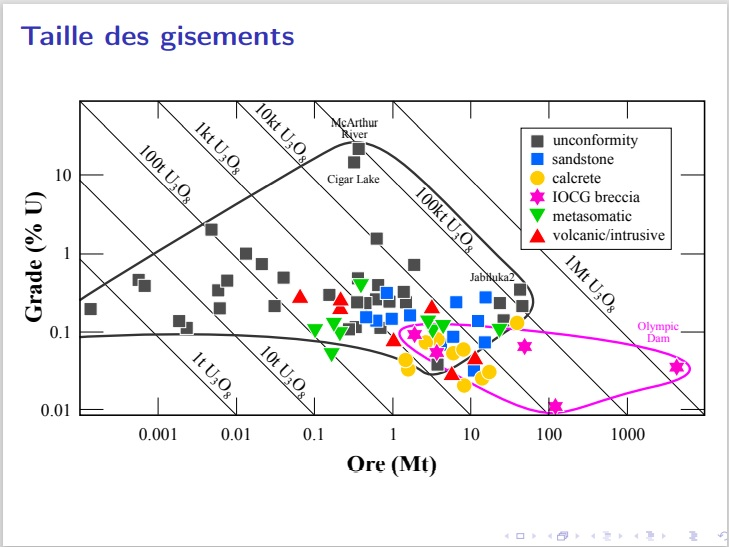
\includegraphics[width = \linewidth]{I_A_1.jpg}
    \caption{Taille des gisements d'uranium selon leur teneur et la quantité de minerai}
    \label{fig:gisements_uranium}
\end{figure}
%Image 1 (prez L. Raimbault)

En France, la volonté d’exploiter l’uranium date de la fin de la Seconde Guerre mondiale. Il s’agit alors d’un enjeu stratégique majeur puisque l’objectif était d’assurer l’approvisionnement en uranium de l’armée, qui en avait besoin pour développer l’arme nucléaire. La première mine d’uranium française a ainsi ouvert en 1948. Avec la décision de développer le nucléaire civil, il a ensuite fallu approvisionner en combustibles les centrales nucléaires pour assurer l’indépendance énergétique du pays. L’épuisement des gisements français et la découverte de gisements bien plus importants à l’étranger, notamment au Niger, entraînent la fermeture des mines françaises. La dernière mine d’uranium ferme ainsi en 2001. Au total, il y a près de 230 sites miniers liés à l’uranium en France, qui ont produit environ 76 000 t en un demi-siècle (une mine française produisait quelques tonnes d’uranium par an). Ces sites sont situés dans le Massif Central ainsi qu’en Bretagne et en Vendée (voir la carte \ref{fig:sites_orano}). Le Limousin est à lui seul à l’origine de près de la moitié de la production française. [M. Descostes]

%    Image 2 (prez Orano C. Benesteau)
\begin{figure}[!h]
    \centering
    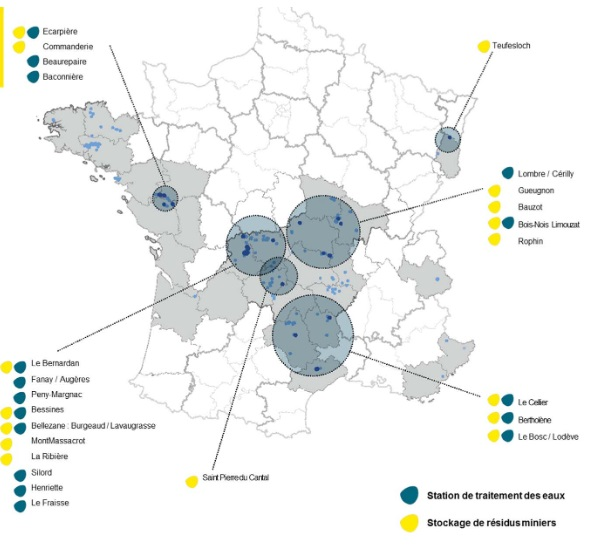
\includegraphics[width=\linewidth]{I_A_2.jpg}
    \caption{Carte des sites miniers uranifères en France.}
    \label{fig:sites_orano}
\end{figure}

Les mines sont régies par différentes autorités : le code minier par exemple, qui pose un cadre juridique récent, ainsi que diverses polices des mines, dont la police des ICPE (installation classée pour la protection de l’environnement), créée en 1976. Des polices liées à des domaines transverses tels que l’eau, les déchets, ou encore la santé, interviennent elles aussi sur ce sujet qui lie ainsi de nombreux domaines. Le RGIE complète enfin ces polices des mines. [IRSN]

Ces polices sont nécessaires car les risques miniers sont importants et peuvent causer de lourds dégâts. On parle d’instabilité mécanique pour désigner les risques d’effondrement ou d’affaissement de pans de mines, ou de rupture des digues de rétention de l’eau. Il y a aussi des risques d’impact sur l’hydrosystème : pollution de l’eau, inondation, ou sur le cycle de l’eau lorsque les eaux qui parcourent le site minier, aussi appelées eaux d’exhaure, sortent à la surface et confluent dans d’autres cours d’eau voisins. Cela arrive souvent après l’abandon d’une mine, et un ruisseau dit d’exhaure se forme alors. Par ailleurs, les travaux miniers souterrains peuvent eux aussi affecter l’hydrosystème si l’eau se propage dans les galeries, voire créer un impact sur l’hydrodynamique même du milieu. [L. Raimbault et E. Ledoux]
%… (transition !)

Nous avons eu l’occasion de visiter virtuellement deux mines d’uranium : la mine de Bellezane et celle de la Ribière. 

Le site de Bellezane comporte en fait deux mines à ciel ouvert. C’est un site en Haute-Vienne qui a été exploité de 1975 à 1992. 5 \% de la production d’uranium français provient du site de Bellezane, qui employait alors jusqu’à 100 personnes. Ce site, qui fait partie de la concession minière de la Gartempe, est un site historique français, de taille conséquente (25 kilomètres de galeries souterraines). De plus, il bénéficie de sa propre station de traitement des eaux, utilisée pour traiter environ 500 000 $\text{m}^3$ d’eau par an. [C. Benesteau]

Le site de la Ribière, abordé plus en détail dans ce rapport, est un site de plus petite taille, avec une teneur plus faible en uranium et un minéral extrait différent (de l’autunite, tandis qu’à Bellezane on extrayait surtout de l’uraninite). Le site, dans la Creuse, avantagé par sa topographie, a été exploité de 1959 à 1984, puis a servi de lieu de traitement de l’uranium faible de 1982 à 1985. C’est, tout comme Bellezane, un site de stockage de résidus uranifères. Contrairement à Bellezane, il n’y a pas de station de traitement liée au site. [C. Chautard]

%Image 3 (prez de Bellezane)            Image 4 (prez de la Ribière)
% \begin{figure}[!ht]
%   \centering
%   \subfloat[]{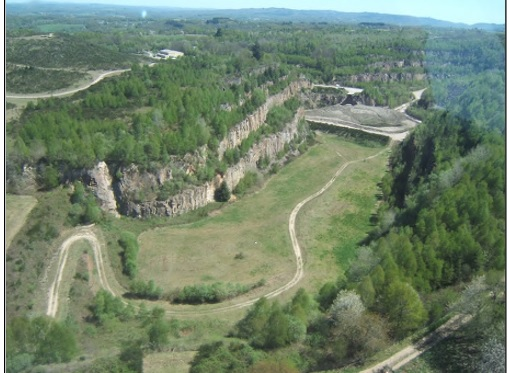
\includegraphics[width=0.4\textwidth]{I_A_3.jpg}}
%   \hfill
%   \subfloat[]{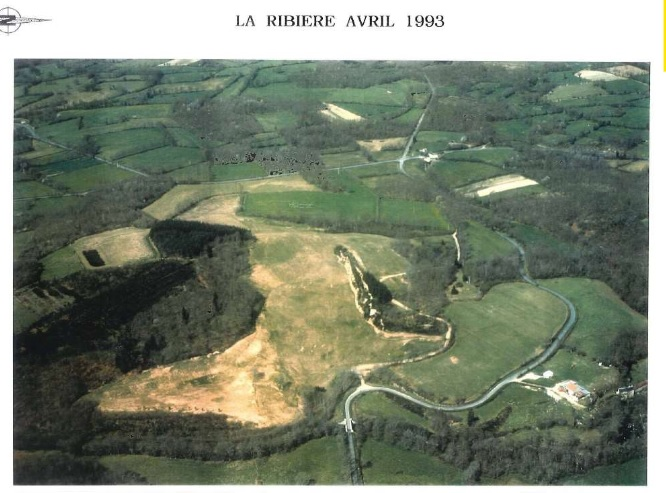
\includegraphics[width=0.4\textwidth]{I_A_4.jpg}}
%   \caption{}
% \end{figure}

\begin{figure}[!ht]
    \centering
    \begin{minipage}{0.5\textwidth}
        \centering
        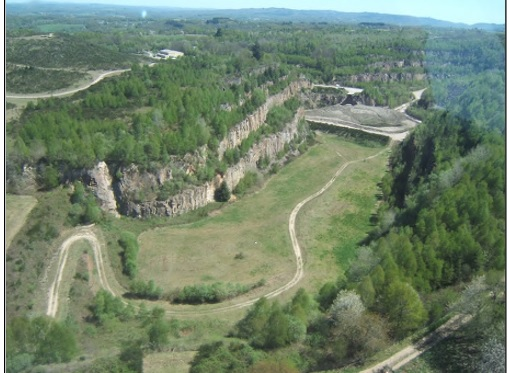
\includegraphics[width=0.9\textwidth]{I_A_3.jpg} 
        \caption{Site de Bellezane. (Orano)}
        \label{fig:bellezane1}
    \end{minipage}\hfill
    \begin{minipage}{0.5\textwidth}
        \centering
        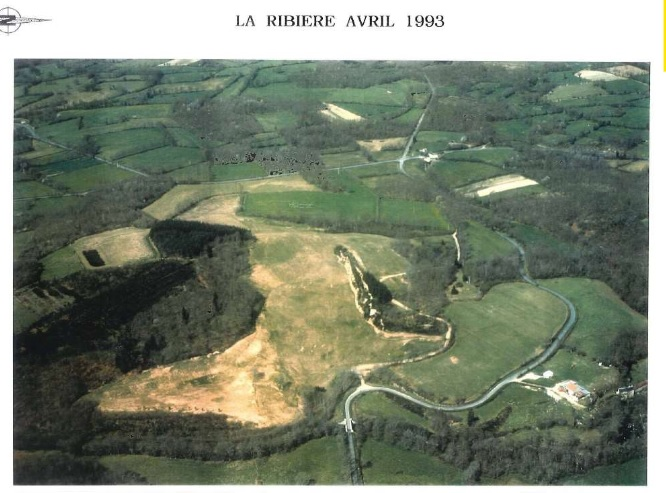
\includegraphics[width=0.9\textwidth]{I_A_4.jpg} 
        \caption{Site de La Ribière. (Orano)}
        \label{fig:ribiere1}
    \end{minipage}
\end{figure}

%%%% GUILLAUME JE FAIS REGARDE : Ok je regarde Au pire viens sur Zoom
% ça a marché 
% nan je peux pas je suis sur zoom sur la conf Ah ok np..... La c'était juste pour mettre 2 trucs cote a cote. Ca devrait pas etre trop courant
% au pire un google rapide hein 
% https://tex.stackexchange.com/questions/5769/two-figures-side-by-side
% je suis pas un expert je fais juste des copiers collers Bah pareil, mais aparemmnt j'avais trouve une autre syntaxe qui marchait aussi
%LJ t'es encore la?
%  oui oui oui oui oui 



A partir de 1967, le nombre de mines tend à décroître. Ce sont les mines de charbon qui disparaissent en premier, puis celles de bauxite, d’argent… À partir des années 1980, ce sont les mines d’uranium qui ferment massivement. Située à Jouac, non loin de Bessines, la dernière mine d’uranium française a fermé en 2001. Pour autant, cette date ne marque pas la fin de l’histoire des mines d’uranium en France. Il s’agit désormais de réaménager les sites de manière durable. C’est ce que l’on appelle l’après-mine.

%Annexe 1 Carte minière de la France 
% et il suffit dans le texte de faire un truc



\subsection{Importance et enjeux de l'après-mine}
\paragraph{} L’après-mine fait partie intégrante du cycle minier. [N. Himeur] Aujourd’hui, cette phase est pensée dès les phases d’exploration et de développement du projet minier. C’est une étape clé qui comporte de nombreux enjeux. Elle dure en général plusieurs dizaines d’années, et il est nécessaire de surveiller la mine même au-delà. Il faut en effet assurer la sécurité et la salubrité de la mine.

L’objectif de ce processus est de réduire l’impact du site sur son environnement. Pour cela, il est essentiel de mettre en place un plan de réaménagement en concertation avec les autorités et les habitants. Une fois le plan établi et les différentes procédures achevées, les travaux peuvent commencer pour réinsérer le site dans le paysage. L’après-mine consiste aussi en la surveillance des sites. A l’issue du réaménagement, il faut continuer à entretenir les équipements de dépollution et vérifier que les normes sont toujours respectées.


%Image 1 (prez Après-mine Orano)
\begin{figure}[!h]
    \centering
    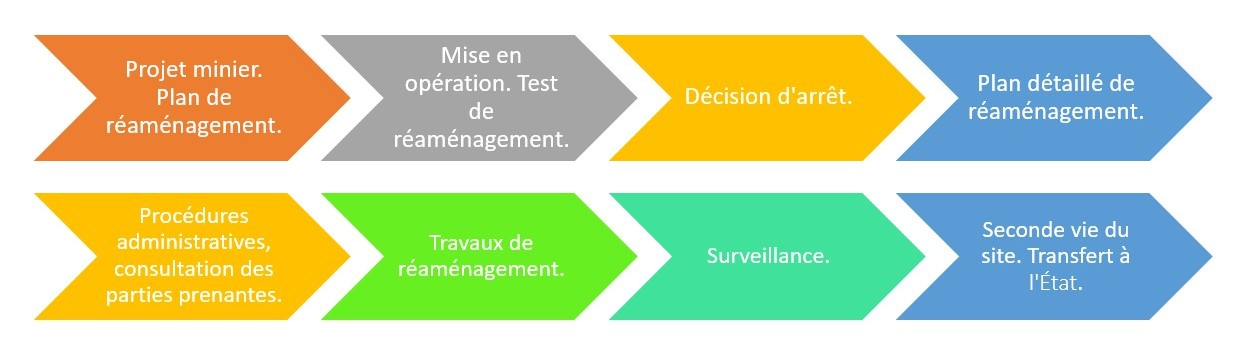
\includegraphics[width=\linewidth]{I_B_1.jpg}
    \caption{Les différentes phases du réaménagement d'une mine. (Orano)}
    \label{fig:phases_reamenagement}
\end{figure}

La roche que l’on a excavé dans une mine pour atteindre le minerai constitue le stérile minier tandis que le produit issu du concassage du filon est appelé résidu minier. Ce dernier garde des propriétés radioactives : il faut donc le stocker et le surveiller.
Pour le réaménagement actif (remblayage), il s’agit souvent d’utiliser les stériles miniers pour remblayer les anciennes mines à ciel ouvert. On peut ensuite revégétaliser la zone - mais attention à ne pas planter d’arbres au-dessus des résidus, car leurs racines pourraient percer jusqu’à ces derniers. Il faut aussi s’assurer de ne pas forcer la nature, qui doit d’elle-même reprendre ses droits. Cela peut alors prendre 6 mois comme au Gabon, ou près de 10 ans comme près de Clisson en France où une forêt maritime est en train de se former. La stabilité peut être assurée avec des digues, qui retiennent les eaux d’exhaure et/ou les résidus. Des contrôles des résidus sont effectués régulièrement ainsi que des analyses de concentrations de radionucléides (uranium, radium…) dans l’eau et l’air du site.  [N. Himeur]

Des stations de traitement des eaux sont souvent utilisées pour traiter les eaux d’exhaure, certaines avec des méthodes de filtration particulières sur résines échangeuses d’ions ou sur zéolites, ce qui sera abordé plus tard dans le document. Le pôle Recherche et Développement (R\&D) de l’exploitant (Orano pour la France) a un rôle à jouer en essayant d’innover, d’optimiser ce traitement et d’étudier l’impact de l’après-mine sur les écosystèmes pour le minimiser. [J. Schick]

Les secondes vies des mines peuvent être diverses : certaines sont transformées en parcs photovoltaïques, en zones industrielles ou agricoles, en réacteur nucléaire naturel comme à Oklo au Gabon, en musée (comme le musée Uréka de Bessines-sur-Gartempes), en base nautique ou encore en parc. Les projets de parc photovoltaïques sont effectués en partenariat avec NEOEN ou via des appels d’offres. [N. Himeur]

À Bellezane, de nombreuses procédures ont été lancées. Des résidus y ont été coulés avant d’y poser une couverture en stériles et terre, puis de commencer la revégétalisation. Il y a notamment sur le site des fourrés et des mares à protéger, un écologue passe donc annuellement sur le site. L’entreprise MISTRI s’est désormais installée dans les anciens locaux du site, et un projet de centrale photovoltaïque en partenariat avec Total est en cours : il devrait aboutir vers 2023. Le stockage des sédiments sur le site est, lui, géré par Orano. [C. Benesteau]

%Image 2  : Bellezane avant/après
\begin{figure}[!hbt]
    \centering
    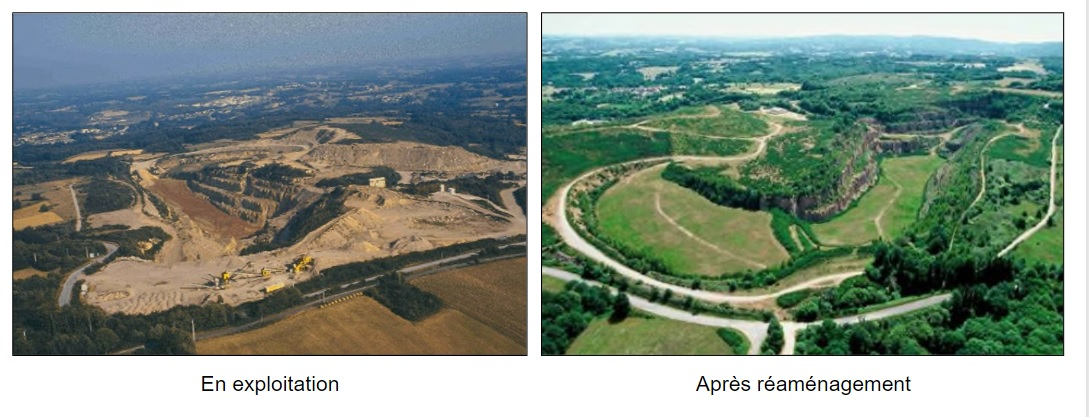
\includegraphics[width=\linewidth]{I_B_2.jpg}
    \caption{Le site de Bellezane avant et après le réaménagement. (Orano)}
    \label{fig:bellezane_avant_apres}
\end{figure}

L’après-mine comprend une dimension sanitaire : les eaux d’exhaure peuvent se déverser dans des lacs ou des nappes utilisés pour le pompage de l’eau potable. C’est le cas par exemple dans le Limousin : les eaux d’exhaure de l’ancienne mine Henriette se déversent dans l’étang de la Crouzille qui est utilisé par la régie de l’eau de la métropole de Limoges pour alimenter le réseau d’eau potable. L’entreprise chargée de l’après-mine, Orano, doit donc veiller à la qualité de l’eau rejetée dans l’étang, qui ne doit pas dégrader la qualité de l’eau de l’étang. La présence de mines est également source de contraintes pour la régie de l’eau : la teneur en métaux et en minéraux de l’eau est modifiée par les eaux d’exhaure ce qui occasionne des frais de surveillance et de traitement supplémentaires. De plus, la disponibilité de l’eau est parfois réduite. Les mines ont également des effets indirects : elles ajoutent des contraintes de gestion technique et suscitent la méfiance des populations à l’égard des gestionnaires de l’eau. [J-L Viallesèche]

En raison des différents risques, notamment sanitaires, l’après-mine fait l’objet d’une réglementation. Celle-ci s’est développée en France dans les années 1970.
 La police des ICPE régie le stockage des résidus et la RGIE (Règlement général des industries extractives) le réaménagement. Ce n’est pas tout : diverses commissions de suivi sont mises en place, en général une par an pour les sites principaux : elles informent le public - notamment les riverains - sur les activités de gestion des sites.
L’IRSN, l’Institut de Radioprotection pour la Sûreté Nucléaire, est un organisme public qui participe aussi à l’après-mine : il réunit des experts scientifiques sur la question, forme et enseigne à des élèves et informe le public. Orano participe également à des congrès, à des études locales et à des groupes de travail sur le sujet. Ces derniers peuvent réunir des acteurs de domaines très divers : Ministère de la Transition Écologique, exploitant (Orano), experts techniques de l’IRSN, du BRGM ou de Geoderis, élus locaux, société civile… Ils étudient différents scénarios en se basant sur des critères et sous critères environnementaux, sociétaux et techniques différents afin de prendre en compte les avis de tous les acteurs.
Des programmes sont aussi mis en place comme le Plan National de Gestion des Matières et Déchets Radioactifs (PNGMDR) qui fixe des objectifs pour l’après-mine. Reconductible tous les  2 ans, son objectif est d’éclairer les autorités sur le réaménagement et le traitement, tout en prenant en compte l’évolution des situations et les contraintes de maintenance et de gestion.  [IRSN]
Par ailleurs, des visites de sites, des présentations et des conférences sont organisées pour sensibiliser et informer le public. Un musée, baptisé Urêka et situé à Bessines-sur-Gartempes, a été inauguré en 2013 dans le but de retracer l’histoire de l’industrie minière uranifère dans le Limousin.

Pour Orano, les mines représentent actuellement près du tiers des activités en France mais cette activité minière consiste principalement à réaménager les sites. Orano est chargé de l’après-mine uranifère en France, ce qui correspond à la gestion de près de 237 sites. Cela représente donc un enjeu important pour Orano : 26 personnes se consacrent à temps-plein à cet après-mine à Bessines-sur-Gartempes, dans le Limousin. Pour l’entreprise, l’après-mine représente 6 millions d’euros de dépenses annuelles pour la surveillance et l’entretien auxquels s’ajoutent 3 à 5 millions d’euros d’investissement dans des projets d’améliorations. Il y a donc également un enjeu économique pour l’entreprise. [N. Himeur]

Orano investit dans des outils spécifiques à l’après-mine afin de permettre un gain d’efficacité, ce qui démontre son importance dans le cycle minier. Des Systèmes d’Information Géographiques (SIG) ont notamment été mis en place, comme ArcGIS. Ce logiciel équipe Orano Mining afin de faciliter les tâches des techniciens chargés de la surveillance des sites. Les relevés sont notamment beaucoup plus rapides et précis grâce à cet outil. Des formulaires disponibles dans le logiciel permettent de recenser en temps réel les anomalies constatées sur le site et s’assurer qu’elles sont résolues par les autres équipes. Les points de prélèvement d’analyses d’eau et d’air y sont aussi indiqués, et les relevés peuvent eux aussi être faits en temps réel. ArcGIS permet de plus d’afficher des zones en réalité augmentée et de guider l’acquisition des données. 

D’autres outils numériques ont été développés pour l’après-mine. CartOmines est une story map permettant d’afficher d’anciennes vues minières (galeries, descenderies…) pour les comparer aux vues actuelles, grâce à d’importantes géodatabases. [CartOmines] Collector permet de modifier des données cartographiques et même de visualiser les galeries des mines en 3 dimensions ou en coupe. Le logiciel ERICA est utilisé pour évaluer les risques générés par l’uranium. Enfin, les bases de données Prodata, ainsi que les logiciels HYTEC et CHESS, que nous avons eu l’occasion d’utiliser, sont des outils importants utilisés pour la modélisation géochimique, hydrochimique et hydrogéologique des sites miniers. Puisqu’ils permettent de gérer l’après-mine en temps réel, les outils ont une grande importance. C’est pourquoi un budget annuel de 100 000€ leur est alloué. [S. Gerland]


%Image 3 (Akkari, S., Willocquet, R., 2020)
\begin{figure}[H]
    \centering
    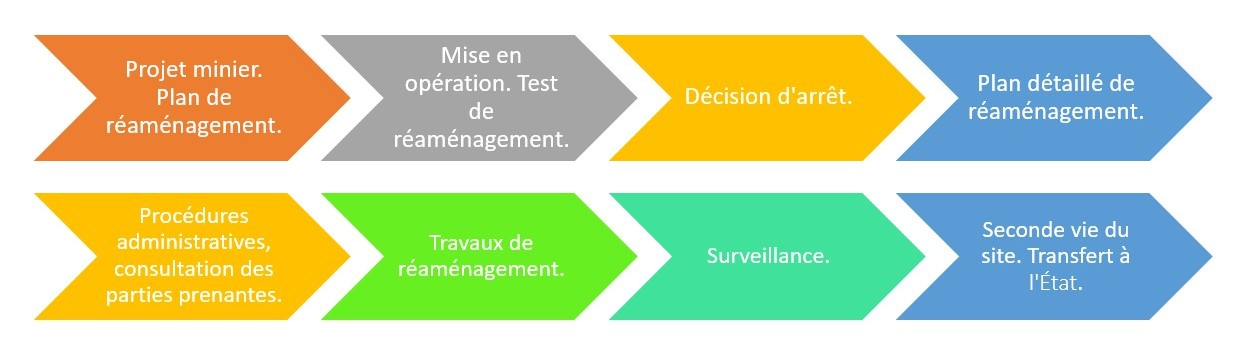
\includegraphics[width=0.9\linewidth]{I_B_3.jpg}
    \caption{Les différents acteurs de l'après-mine. (Willocquet, R., Akkari, S., 2020)}
    \label{fig:acteurs_apres_mine}
\end{figure}

Ainsi, l’après-mine répond à de nombreux enjeux : il faut gérer les résidus et les stériles miniers, gérer les eaux d’exhaure, assurer la stabilité mécanique du site, surveiller l’impact radiologique, sans oublier la dimension sociale : le projet doit être accepté par les habitants et doit s’inscrire dans un projet de réhabilitation sur le long terme. Enfin, pour l’exploitant, il y a aussi une dimension économique.

\subsection{Enjeux sanitaires de l’Après-Mine}
\paragraph{Uranium}

Les différentes organisations de riverains et les acteurs publics en France se focalisent surtout sur la dangerosité de l’uranium. Pourtant, en ce qui concerne cet élément, il y a très peu d'études sur l’impact des mines sur la santé publique. Par exemple, au Québec, seulement 11 études ont été retrouvées par l’institut national de santé publique du Québec, ce qui n’est pas suffisant pour donner de vraies conclusions sur les effets des résidus miniers. De plus, les études menées ne prennent parfois pas en compte le bruit de fond pour donner leur conclusion et sont donc inutilisables. Le bruit de fond correspond à la radioactivité présente naturellement dans les roches. Elle varie selon les contextes géologiques. En France, afin d’étudier l’impact de l’uranium sur la santé humaine, l’IRSN se base sur des études sur l’influence d’un fort dosage d’uranium sur la santé des rats et a mis en évidence un effet délétère sur certains organes comme le cerveau ou les reins. 


Les sources les plus intéressantes de mise en évidence des effets sur la santé humaine proviennent d'études sur des individus étant régulièrement en contact de cet élément. Par ailleurs, des études sur les anciens mineurs ont mis en évidence que les cas de cancer du poumon étaient 127\% de fois plus élevés que la moyenne française. 
Il est avéré que l'uranium est à la fois chimiotoxique et radiotoxique. Les effets les plus importants sont observés au niveau des reins, avec atrophie tubulaire et amincissement du cortex rénal.

\paragraph{Radon}

Une autre source de pollution potentiellement dangereuse pour l’homme est le radon. Celui-ci est un gaz nocif pour l’humain. Les principales études sanitaires sur ce gaz ont été menées dans les années 1920. D’après elles, une exposition chronique au radium par ingestion peut causer non seulement des anémies mais aussi des cancers et une détérioration des tissus du squelette.
Plus récemment, l’IRSN a mené une étude sur le lien entre l’augmentation du taux de décès par cancer du poumon et la présence de radon dans les maisons. Les résultats ont été publiés en 2004 dans la revue « Epidemiology » [Baysson et al 2004]. Ils montraient une augmentation faible du risque de cancer du poumon associée à l’exposition au radon  domestique. Cependant, les résultats sont très peu fiables étant donné qu’ils ont donné des résultats à la limite de la significativité statistique.  

\paragraph{Autres polluants}

Alors que l’on a tendance à se focaliser sur l’uranium et le radium dans l’étude des anciennes mines d’uranium, il ne faut pas oublier que l’on observe dans les mines la présence d'autres métaux qui peuvent être nocifs pour l’homme. Il y a par exemple le fer qui peut être trouvé à des concentrations assez élevées, lié à la présence d'oxydes de fer dans le milieu.  L'inhalation de concentrations excessives d'oxyde augmente le risque de développement de cancer du poumon, particulièrement pour les ouvriers exposés. Le plomb nuit également au système sanguin, au système nerveux, et au système rénal.
L’aluminium a quant à lui un impact sur le système osseux et sur le système nerveux. Cependant, d’après Santé Publique France, la détermination de l'impact sur la santé de l'exposition humaine à l'aluminium reste encore extrêmement difficile et source de nombreuses controverses. Une étude a été menée par l’Agence Française de Sécurité Sanitaire et a mis en évidence que l’aluminium pouvait avoir un impact négatif sur l’environnement et les hommes mais sans pouvoir définir précisément les impacts.  Par exemple, des effets neurologiques de l’aluminium sur l’humain ne se sont pas retrouvés avérés.

\newpage
\section{Problématique de l’Après-Mine}
\subsection{Les différentes pollutions}

 
\subsection{La dimension sociétale}
\subsubsection{Focalisation du grand public sur l'uranium et les risques radiologiques}
\paragraph{} Le manque d’informations transmises par COGEMA (\emph{COmpagnie GÉnérale des MAtières nucléaires}) lors du début du réaménagement des mines a rendu la population locale méfiante envers les différentes actions que l’entreprise a prises pour enfouir les déchets radioactifs. Alors que COGEMA affirmait avoir été transparent sur leur gestion des déchets, certains journalistes indépendants accusent l’entreprise d’avoir enfoui des bidons dans les résidus miniers sans prévenir ni alerter les riverains. 

De nos jours, des tensions sont encore présentes entre Orano et les riverains. De nombreuses associations se sont formées pour protester contre la “mauvaise gestion de l'après-mine” (Collectif Mines d’Uranium). Le collectif \emph{Mines d’uranium} (regroupant plusieurs associations dont \emph{Oui à l'avenir} (Creuse), \emph{Noria} (Vendée), \emph{Sources et Rivières du Limousin}, et bien d’autres) déplore l’état dans lequel les entreprises minières laissent le territoire et  affirme que les déchets miniers sont souvent “disséminés dans l’environnement ou stockés dans des conditions totalement inappropriées” et qu’ils “génèrent des pollutions environnementales multiples (air, eau, sol, chaîne alimentaire) induisant des dangers sanitaires inacceptables aujourd’hui et pour les générations futures” (Collectif Mines d’Uranium). 

% rewording à faire

Ils tiennent Orano pour responsable de la dégradation de la faune et de la flore et protestent contre une “législation complaisante”. Ils se plaignent, entre autres, de la contamination des terrains par des éléments radioactifs, de la pollution des ressources aquatiques, de la mauvaise gestion des sites de stockage des déchets, de la perte de mémoire sur la localisation des sites, de l’absence de normes sanitaires et environnementales intégralement respectées… 


Les associations ne se contentent pas d’informer la population sur les risques inhérents aux anciennes mines. L’association CRIIRAD (Commission de Recherche et d’Information Indépendantes sur la Radioactivité)  contrôle également la radioactivité de l’environnement pour évaluer l’impact des déchets radioactifs. En 2004, une action de contrôle de radioactivité les a amenés à prélever des échantillons au bord d’un ruisseau en aval d’un ancien site minier. La radioactivité mesurée dans ces échantillons était de 3,4 Bq/g, soit d’après leur chiffre trois fois plus que la teneur naturelle. Selon eux, le fait qu’il n’y ait plus de contrôle radioactif officiel autour des mines est un danger pour l’environnement et pour la vie humaine. 


\subsubsection{Gestion des risques par un acteur extérieur: rôle de l’IRSN}
Plus spécifiquement en ce qui concerne les risques liés à la radioactivité, l'Institut de Radioprotection et de Sûreté Nucléaire (IRSN), est un Établissement Public à caractère Industriel et Commercial créé en 2001 qui fonctionne sous la tutelle conjointe des ministères de la Défense, de l’Environnement, de la Recherche de la Santé. Il s’agit de l’expert français en matière de recherche et d’expertise sur les risques nucléaires et radiologiques. L’IRSN s’intéresse à l’impact radiologique sur la santé et sur l'environnement et intervient dans la gestion de la sûreté et de la sécurité nucléaire.  Lors de la prise en charge d’un projet comportant un risque radiologique, l’IRSN, les concepteurs ou constructeurs, les autorités publiques et les parties prenantes (comme les Commissions Locales d’Informations) sont en interaction mutuelle.

L’IRSN s’occupe donc  du réaménagement des anciennes mines d’uranium en France. Pour ce faire, l’institut doit tout d’abord connaître l’impact radiologique de l’ancienne mine sur l’environnement et sur les populations. Le modèle ERICA (méthode d’évaluation du risque environnemental associé aux rejets de substances radioactives mise en place dans le cadre du projet européen ERICA) est utilisé pour déterminer  le risque environnemental en effectuant des mesures dosimétriques sur le terrain. L’objectif est de quantifier la probabilité de l’existence d’un risque potentiel sur les écosystèmes aquatiques.

L’institut  mène  des  expertises  afin  d’évaluer  des  points  techniques  particuliers,  concernant notamment l’impact radiologique de certains sites. Lorsqu’elles sont réalisées à la demande des préfets, les interventions de l’IRSN prennent en général la forme de tierces expertises, portant sur les documents techniques produits par Areva au sujet des travaux qu’il mène sur  ses  sites  ou  de  l’impact  environnemental  de  ceux-ci.

Pour les sites miniers, l’enjeu est le long terme: les polluants seront là pendant des dizaines de milliers d’années. Les réglementations qui s’appliquent sur ces sites sont le code de la santé publique, pour la protection du public contre les rayonnements ionisant autour des anciens sites miniers d’uranium; le code minier, pour la partie exploitation, surveillance et réaménagement; et le code de l’environnement, pour le stockage des résidus.

L’objectif pour les entreprises est de faire en sorte que les eaux rejetées dans l’environnement   soient conformes aux limites fixées par arrêté préfectoral. Il est  basé sur les limites fixées par le RGIE (Règlement Général des Industries Extractives).

Au niveau sanitaire, l’impact radiologique sur la santé a été évalué par la Commission Internationale de Protection Radiologique qui a évalué le risque à 17 cancers pour 100 000 personnes exposées à 1 mSv/an. La limite fixée pour le public est de 1 mSv/an et pour les travailleurs miniers de 20 mSv/an. Or, certains acteurs comme des associations pour les travailleurs au Niger ou les "Amis de la Terre” en France dénoncent Orano pour ne pas avoir admis mettre en danger ses travailleurs en les exposant à 20 mSv/an. Selon eux, d’une part les études scientifiques ne sont pas précises et donc Orano n’est en rien obligé de se plier aux seuils définis par la CIPR et d’autre part Orano ne prend pas en compte dans ses calculs les émissions radiologiques liées au fond géochimique lorsque le travailleur rentre chez lui.

\subsection{Les différentes normes mises en place sur l’eau}
\subsubsection{Acteurs de la législation}
\paragraph{} De nombreux acteurs interviennent dans la mise en place d’une législation régissant la qualité des eaux. Tout d’abord, c’est l’Union Européenne qui établit des directives. Les états-membres doivent transposer ces actes juridiques dans leur législation nationale. En France, le  ministère de l’environnement contrôle le Comité National de l’Eau, qui évalue la qualité et le prix de l’eau, et l’Office National de l’Eau et des Milieux Aquatiques  qui contrôle les usages des milieux aquatiques. Il existe aussi des institutions régionales : la direction régionale de l’environnement, de l’aménagement et du logement, l’agence régionale de santé et la direction départementale du territoire  appliquent les directives nationales dans les différents régions. De manière encore plus locale, les collectivités territoriales (communauté de communes ou d’agglomérations, métropoles) donnent des ordres pour les travaux de Gestion des Milieux Aquatiques et de Prévention des Inondations. Enfin, les acteurs économiques et les diverses associations de protection de l’environnement entrent en jeu : les industriels et les agriculteurs sont responsables de leurs installations de dépollution et de prélèvement. Parallèlement, les associations sont associées aux décisions au sein du Comité de bassin, appliquées par l’agence de l’eau.

\subsubsection{Cas de l’eau rejetée dans l’environnement}
Lorsqu’il n’est pas nécessaire que l’eau soit potable, la DCE (Directive-Cadre sur l’Eau) est la directive européenne qui fait loi. Adoptée en 2000 pour préserver la ressource en eau, elle indique des valeurs seuils pour protéger la vie humaine mais aussi l’environnement. Les NQE (Normes de Qualité de l’Eau) sont définies dans la DCE au niveau européen pour les substances polluantes prioritaires. La NQE est la plus faible des PNEC (“Predicted No Effect Concentration”) : concentration en dessous de laquelle aucun effet inacceptable n’est observé. Ces NQE n’étant définies que pour les polluants considérés comme prioritaires, des VGE (Valeur Guide Environnementale) ont été établies: elles sont calculées comme les NQE mais n’ont pas de valeur réglementaire (donc ne sont pas obligatoirement respectées).

Pour définir ces normes, il faut notamment prendre en compte le fond géochimique. Le fond géochimique est la composition chimique d'un sol et des roches du sous-sol dont il est la décomposition. Il détermine en partie la qualité du sol, de l'eau et la vie de la flore et de la faune. On distingue généralement le fond géochimique naturel, résultant exclusivement de l'évolution de la roche-mère et d'apports naturels : salinité, confinement d’une eau, phénomène de drainance, et le fond d'origine anthropique, qui exprime la part des éléments exclusivement introduits dans le milieu par les activités humaines ou à la suite de ces activités. Le fond géochimique naturel est parfois confondu avec le  “bruit de fond”, mais ce dernier comprend également des apports anthropiques diffus. Les substances généralement considérées pour l’évaluation d’un fond géochimique sont  l’arsenic, le baryum, le bore, le fluor, le cadmium, le chrome, le mercure, le cuivre, le nickel, le plomb, le zinc, l’antimoine, le sélénium, l’aluminium, l’argent, le fer et le manganèse.

Pour quantifier la quantité de polluants dans le milieu, les différents acteurs ont besoin de connaître le fond géochimique du milieu afin de savoir s’ils dépassent sa valeur pour les polluants lors du rejet des eaux dans l’environnement. Or, ce bruit de fond géochimique est difficile à quantifier car il dépend du milieu, et au sein d’un même site sa valeur peut varier d’un point à un autre. Les acteurs ont alors du mal à quantifier la quantité de polluants qu’ils rejettent dans l’environnement et peuvent parfois dépasser les valeurs seuils en prenant en compte une valeur de bruit de fond géochimique plus importante. De plus, la proportion naturelle en certains éléments est parfois supérieure à celle fixée par la législation. C’est en France le cas du baryum (concentration maximale naturelle de 1600 mg/L alors que la norme est à 700 mg/L), du fluor (12 g/L contre 1.5 g/L) ou encore du nickel (100 mg/L contre 20 mg/L) par exemple. D’où la difficulté à établir des normes qui puissent être respectées partout. %/ cf tableau

Un autre moyen pour établir l’impact de la pollution des eaux de surface sur l’environnement est d’étudier la faune et la flore du milieu. Cela pose un problème car les effets sont donc observés après la pollution du milieu et peuvent ne pas être pris en compte par les entreprises. 

\subsubsection{Cas de l’eau potable} 

\paragraph{} Lorsque l’eau est destinée à la consommation humaine, les critères de potabilité sont établis sur la base des recommandations en vigueur de l’Organisation Mondiale de la Santé (OMS) et sur celle de données scientifiques établissant des doses maximales admissibles (DMA), définies comme la quantité maximale d’une substance qu’une personne peut absorber tous apports confondus (alimentaires, hydriques), sans danger, chaque jour, sa vie durant. Ces doses sont calculées pour des personnes fragiles (bébés, femmes enceintes, immunodéprimés).

Ces critères sont basés sur les principaux indicateurs de la qualité de l’eau. Ils indiquent les  germes pathogènes, virus et bactéries, micro-organismes parasites ainsi que les autres polluants chimiques à éliminer, et de même quels sels minéraux et quels oligo-éléments sont à conserver (comme le calcium, le magnésium, le chlore ou le fer). Afin de fixer une réglementation adaptée, une différence fondamentale est établie entre références de qualité et normes de qualité: les normes de qualité, impératives, concernant des substances pouvant avoir une répercussion sur la santé tandis que les références de qualité (couleur, odeur) sont des indicateurs reflétant le bon fonctionnement des installations de production d’eau potable.
La qualité de l’eau potable est encadrée par une réglementation européenne, le Code de la Santé publique, des décrets, des arrêtés, des circulaires et en particulier par la Directive européenne 98/83 du 3 novembre 1998 et par  le décret 2001-1220 qui fixe les limites et références de qualité pour l’eau potable. Plus spécifiquement, en France, le code de santé publique (CSP) régit le socle de la réglementation en matière de qualité, de production et de distribution de l’eau et transpose les directives européennes. 

\subsubsection{Comparaison avec d’autres pays}

\paragraph{Australie}

En Australie, les \textit{Environmental Requirements} (ER) pour la mine d’uranium de Ranger, établis en 1999, fixent les normes de protection environnementale auxquelles l’entreprise responsable d’un site minier doit se soumettre. L’entreprise doit s’assurer que les opérations minières ne compromettent pas l’écosystème environnant et la santé de la population locale. Elle doit maintenir la biodiversité des écosystèmes et assurer la continuation des processus biologiques. Elle doit par ailleurs réhabiliter le site minier de sorte à établir un environnement correspondant à sa zone géographique, en assurant la revégétalisation avec des espèces natives de cette zone, avec la même densité et abondance, ou encore en faisant en sorte que les caractéristiques d’érosion du site soient cohérentes, afin d’assurer la viabilité à long terme et, à terme, de permettre à la zone de se développer sans maintenance particulière par rapport aux zones alentour. De plus, l’entreprise doit assurer des conditions radiologiques stables afin que la dose reçue par les travailleurs et le public soit aussi basse que raisonnablement possible. Elle doit pour cela minimiser le volume d’eau contaminée nécessaire pour faire fonctionner le site, et minimiser la quantité de contaminants présente dans cette eau, tout en s’assurant que ces contaminants soient contenus dans le site. De même, les émissions gazeuses et particulaires doivent être minimisées. L’objectif étant de limiter autant que raisonnablement possible les risques pour la santé des locaux. L’entreprise doit pour cela suivre le principe BTP (\textit{Best Practicable Technology}), en implémentant la technologie disponible ayant le plus de retombées positives sur l’environnement. L’Australie a donc mis en place un mode de gestion ALARA (\textit{As Low As Reasonably Possible}) pour le contrôle et la réhabilitation de ses mines d’uranium.
Les mesures correctives doivent être prises en accord avec le ministère de l’environnement, mais ce sont les compagnies minières qui ont la responsabilité de réaliser la réhabilitation et de payer les coûts associés jusqu’à ce que les autorités (comme par exemple le Northern Territory Department of Mines and Energy: NTDME) estiment que le site a été réhabilité à un niveau satisfaisant. La surveillance du site doit par ailleurs s’effectuer par des prélèvements réguliers sur les eaux souterraines.

\paragraph{Allemagne}

En Allemagne, le \emph{Radiation Protection Act} (StrlSchG), établi en 2017, fournit le cadre juridique de la protection face aux effets néfastes des radiations et établit les bases légales de la radioprotection. Cet acte implémente la directive 2013/59/Euratom du conseil européen qui met en place des standards de protection face à l’exposition aux radiations. Cet acte met donc en place des valeurs limites de concentration d’activité, d’activité et de dose effective annuelles précises pour des espèces radioactives et des publics distincts. 


Par exemple, la limite générale de la dose effective annuelle pour le public est de 1 mSv, et la concentration d’activité de l’uranium ne doit pas dépasser 10 kBq/kg. Cependant, il n’existe pas de loi spécifique à la gestion des mines d’uranium après la fin de leurs activités, pas de législation globale sur les méthodes à appliquer. Le gouvernement allemand préfère appliquer des méthodes distinctes pour chaque site afin d’apporter des réponses adaptées à des questions spécifiques.

La réhabilitation des mines d’uranium allemandes est principalement gérée par la société Wisbut GmbH, détenue et financée par le gouvernement. Elle est chargée du démantèlement des mines, du traitement du site et de la surveillance des installations et des émanations. La surveillance implique des mesures menées sur le long terme à des positions précises afin d’assurer la cohérence du site avec la loi et un meilleur contrôle sur les actions de réhabilitation.

\paragraph{Etats-Unis}

Aux États-Unis, en 1950, le US Public Health Service commençait une étude sur les mineurs d'uranium, conduisant à la première publication d'une corrélation statistique entre le cancer et l'extraction d'uranium, publiée en 1962. Le gouvernement fédéral a finalement réglementé la quantité standard de radon dans les mines, fixant le niveau à 0,3 WL en 1969. 

Plus tard, l'USAEC (United States Atomic Energy Commission) a donné l’objectif et des conseils pour la réhabilitation de l’eau dans les anciens sites miniers, surtout pour les eaux souterraines contaminées par l'ISR. L’objectif est de restaurer la qualité de l'eau dans les nappes aquifères affectées à l’état avant l'exploitation minière. Bien que toutes les caractéristiques chimiques ne puissent pas être retournées à celles avant l'extraction, l'eau doit être assurée aux mêmes utilisations qu'auparavant. 

USAEC formule des recommandations concernant la caractérisation du niveau de base (baseline) de la qualité des eaux souterraines avant le début des opérations minières, la surveillance pour détecter l’évolution de lixiviat pendant l'exploitation minière et la surveillance à long terme pour déterminer à quel moment la qualité des eaux souterraines se stabilise après la fermeture des opérations minières.

L'eau avant l'exploitation est généralement de mauvaise qualité (teneurs élevées en métal, en uranium et parfois de haute salinité), résultant des mécanismes de genèse du minerai. L'objectif de qualité physico-chimique à atteindre dépend de la réglementation locale, généralement de concentration aussi proche que possible du niveau de base.

Par exemple, au Texas, c’est la TCEQ (Texas Commission on Environmental Quality) qui définit le niveau de base pour ses sites miniers locaux et surveille la réhabilitation. Le tableau suivant résume les données de référence des eaux souterraines avant l'extraction. Au Texas, 26 éléments chimiques sont mesurés avant l'exploitation minière pour établir le niveau de base, qui est l’objectif initial de restauration. On sélectionne la concentration moyenne la plus élevée de la zone de mine. Dans le site Zamzow, 0,171 milligramme par litre d'uranium était la valeur moyenne la plus élevée de cette zone.

%Figure 2 – Niveau de base du site Zamzow
\begin{figure}[H]
    \centering
    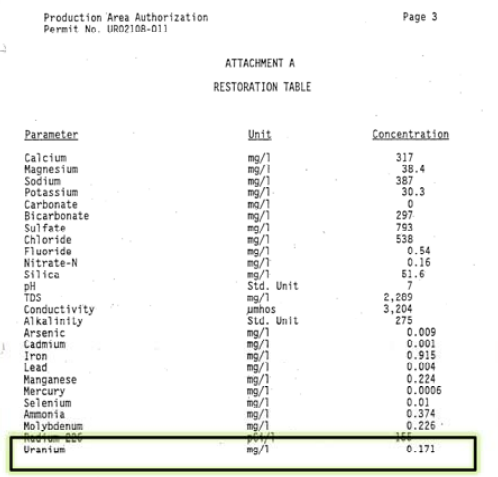
\includegraphics[width=0.8\linewidth]{II_C_2.png}
    \caption{Niveau de base du site Zamzow}
    \label{fig:site_zamzow_base}
\end{figure}

Cependant, une étude publiée par l'U.S. Geological Survey en 2009 a révélé que « À ce jour, aucune opération après ISR aux États-Unis n'a réussi à restaurer l'eau dans l'aquifère au niveau de base ». Tous les sites du Texas ont reçu des objectifs de restauration modifiés pour au moins un élément, déterminés par TCEQ. Les données de restauration finale pour Zamzow montrent une limite modifiée de 3,00 milligrammes par litre pour l'uranium. 


%Figure 3 - Données de restauration finale du site Zamzow
\begin{figure}[H]
    \centering
    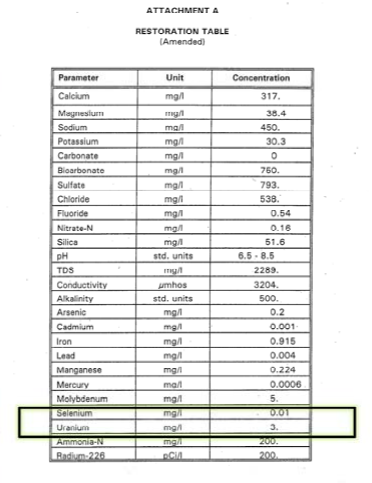
\includegraphics[width=0.7\linewidth]{II_C_3.png}
    \caption{Données de restauration finale du site Zamzow}
    \label{fig:restauration_finale_zamzow}
\end{figure}


Ce graphique de concentration d'uranium pour divers sites du Texas illustre la relation entre les niveaux de base, les valeurs finales après réhabilitation et les objectifs de restauration modifiés. Les barres bleues représentent les niveaux de base. Les barres rouges représentent les concentrations finales pour l'uranium, et les barres vertes représentent les objectifs de restauration modifiés par TCEQ.

%Figure 4 - Concentration d'uranium pour divers sites du Texas

\begin{figure}[H]
    \centering
    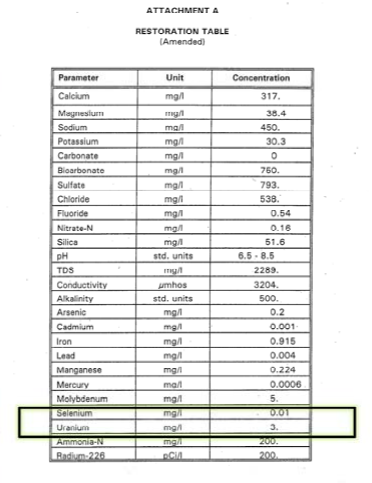
\includegraphics[width=\linewidth]{II_C_3.png}
    \caption{Concentration d'uranium pour divers sites du Texas}
    \label{fig:conc_u_texas}
\end{figure}

\newpage

\paragraph{Canada}

Le Canada est un État fédéral et la responsabilité de la réglementation de traitement et la réhabilitation est partagée entre les gouvernements provincial et fédéral. Le 30 juin 1996, la dernière mine de la région d'Elliot Lake, la mine Stanleigh, était fermée. Après, seule la province de la Saskatchewan produit de l'uranium, mais comme la teneur en uranium du gisement de la Saskatchewan est élevée, le Canada restera le plus grand producteur d'uranium au monde.

L'AECB (Atomic Energy Control Board), un organisme indépendant du gouvernement du Canada, est responsable des affaires liées à l'énergie nucléaire et aux matières radioactives. Le règlement R-90 traite de la fermeture et de la réhabilitation des sites. Bien que le Canada réglemente les mines d'uranium, les provinces sont les principaux propriétaires fonciers. Par conséquent, les mines d'uranium fermées reviendront finalement aux provinces ou redeviendront des terres de la Couronne. Les agences environnementales provinciales sont les principaux régulateurs de la qualité de l'eau de tous les sites miniers.

En 1996, l'AECB a établi la réglementation stratégique de gestion des déchets radioactifs pour s'assurer que les déchets après les mines sont gérés de manière responsable. Les objectifs de cette réglementation canadienne sont :
\begin{itemize}
    \item protéger l'environnement, en tenant compte des facteurs sociaux et économiques
    \item minimiser le besoin de contrôle et de surveillance à long terme
    \item s'assurer que les risques pour la santé sont conformes aux normes en vigueur 
    \item ne pas interdire l'utilisation future des ressources naturelles contenues dans les déchets miniers.
\end{itemize}

Cela signifie en fait que des normes spécifiques sont développées, dépendant des situations actuelles de chaque site. Néanmoins, un certain nombre de critères communs sont applicables à tous les sites. Par exemple, une valeur de 1 mSv par an pour l'équivalent de dose efficace moyen est à respecter sur une période de 50 ans après la fermeture des sites d'uranium, ainsi que les autres exigences légales sur la sécurité nucléaire et la protection radiologique mises en place par AECB.

Dans ce cadre, les propriétaires des déchets sont responsables du financement, de l'organisation, de la gestion et de l’élimination des installations. Pour les anciennes mines d'uranium, dont beaucoup ont été fermées il y a plus de 50 ans, plusieurs facteurs doivent être pris en compte. Dans de nombreux cas, l'entreprise qui exploitait la mine, ou son successeur, existe toujours et s'occupe des déchets sur ses sites. Cependant, dans certains cas, le site est retourné à la Couronne lorsque les entreprises n’existent plus et alors la responsabilité de traitement des déchets est partagée entre les gouvernements provincial et fédéral. Lorsque ces anciennes mines fonctionnaient, les réglementations environnementales appliquées à l'industrie minière n'étaient pas très strictes. Cependant, il n'est pas souvent pratique ou rentable de remettre en état les anciens sites en respectant les normes actuelles. La plupart des sites présentent un risque très faible, en raison des faibles teneurs de minerai, de leurs emplacements éloignés et du fait que les polluants se sont dissipés au cours des 50 dernières années.

\newpage
\section{Traitements/Solutions}
\subsection{Différents traitements}
Le traitement des eaux en sortie de mines est ainsi un enjeu central de l’après-mine. En France, plusieurs techniques de traitement sont utilisées dans les quinze stations stations dédiées. Elles diffèrent par les installations qu’elles requièrent tant que par leurs implications socio-économiques.

\subsubsection{Fonctionnement et coûts}
\paragraph{Traitement par précipitations} \hspace{1 em}

%(IMAGE $III_A_1$)



\begin{figure}[H]
\centering
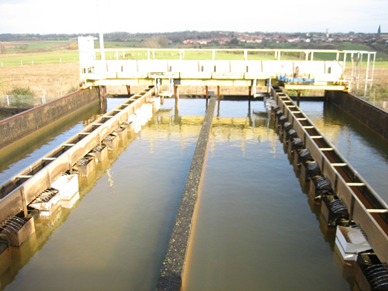
\includegraphics[width = 0.5\linewidth]{III_A_1.png}
\caption{Bassin de décantation}
\label{fig:bassin_decantation}
\end{figure}



Le procédé de traitement des eaux le plus répandu en France est le traitement actif par précipitation et coagulation-floculation-décantation. Il équipe onze des quinze stations de traitement des eaux de sortie de mine françaises. 
L’étape de précipitation vise la transformation des métaux dissous dans l’eau (généralement fer, aluminium, uranium, radium) en précipités insolubles par l’ajout de réactifs, souvent de la chaux ou de la soude, selon la réaction suivante :   
$$Me^{n+} + n(OH) \rightarrow Me(OH)_{n}$$
          	
L’ajout de sulfate d’alumine permet la formation d’hydroxyde d’aluminium susceptible de fixer l’uranium. De même, l’utilisation de chlorure de baryum permet de piéger de radium par la création d’un co-précipité baryum-radium. Ces réactions s’accompagnent d’une augmentation du pH. Etant donné que le pH favorisant la précipitation est différent selon les polluants, il faut ajuster le pH à une valeur optimale en fonction des polluants à éliminer, par exemple par l’ajout de soude ou de chaux.  

La coagulation-floculation consiste en l’agrégation des précipités non décantables en microflocs puis en flocs  pour permettre leur décantation. Les réactifs couramment utilisés à cette fin sont la chaux pour la coagulation et les polymères organiques à longue chaîne carbonée pour la floculation. 

Enfin, la décantation consiste à séparer les phases eau et flocs. Elle peut se faire par passage des effluents dans plusieurs bassins successifs, ou par passage à travers un lit de boue. Les eaux à la surface des décanteurs sont évacuées et les boues créées chargées en polluants sont récupérées au fond des cuves pour être déshydratées puis traitées.

Ce procédé est largement répandu pour le traitement industriel d’eaux riches en métaux. Il nécessite de nombreuses installations pour contenir les matières (cuves de préparation ou de stockage des réactifs nécessaires aux différentes étapes, cuves de précipitation, coagulation, décantation), pour traiter les déchets formés (filière de traitement des boues) et contrôler les caractéristiques des eaux en réaction comme en sortie (mesure de la stoechiométrie, du pH…). 

La maintenance nécessaire pour un site de traitement se divise entre le nettoyage préventif du site à hauteur de douze heures hebdomadaires et l’étalonnage des dispositifs de mesure à hauteur d’une demi-heure hebdomadaire. En prenant également en compte de la consommation énergétique du site (pompes à boues, agitateurs à cuves…) et du prix des réactifs, le prix de traitement d’un mètre cube d’effluent par précipitation-coagulation-floculation varie entre 0,20 € et 0,50 € en fonction des réactifs utilisés.

\paragraph{Traitement par résines échangeuses d’ions} \hspace{1 em}


%(Image $III_A_2$)
\begin{figure}[H]
\centering
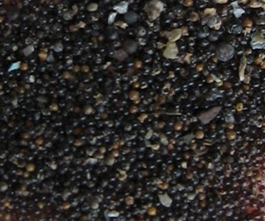
\includegraphics[]{III_A_2.png}
\caption{Une résine échangeuse d'ions}
\label{fig:resine_echangeuse_ions}
\end{figure}

Les résines échangeuses d’ions sont des macromolécules granulaires insolubles. Elles possèdent des radicaux capables de permuter avec certains ions d’une solution de manière réversible. Lors du traitement, la résine se trouve dans un réservoir cylindrique fermé sous pression relié à un filtre et alimenté par un dispositif collecteur du liquide à traiter. Cet ensemble est appelé colonne.

Le processus de traitement consiste à remplacer les ions centraux de complexes polluants par un autre type d’ion qui rendra le nouveau complexe inerte. Il existe 2 types de résines échangeuses d’ions : les résines cathodiques qui remplacent les cations des complexes de la solution (comme l’uranium $\text{U}^{4+}$) par des cations inoffensifs présents sur ces radicaux ; et les résines anodiques qui permutent des anions de la même manière.
L’échange se fait selon l’équation suivante, de manière réversible sans altération ni solubilisation:
$$R-A^+ + B^+ = R-B^+ + A^+$$
R est le radical de la résine, A l’ion de la résine fixé sur ce radical, et B l’ion à éliminer de la solution.

Le traitement se décompose en plusieurs étapes. Si l’espèce polluante n’est pas sous forme ionique, ou si l’eau contient trop de précipités, une élution est nécessaire. L’eau à traiter est ensuite envoyée grâce à une pompe dans le réservoir jusqu’à saturation de la résine. Ce réservoir est ensuite remplacé et transporté jusqu’au lieu de régénération de la résine, où est opéré le procédé inverse du traitement. L’injection d’une solution régénérante permet de remplacer les ions polluants (comme les ions uranium) par de nouveaux ions inertes. Les résines sont ensuite rincées à faible puis fort débit afin d’éliminer les traces de la solution régénérante. Elles peuvent ensuite être réutilisées pour le processus de traitement de l’eau.

Les réservoirs contenant les résines peuvent être disposés en série, pour augmenter l’efficacité du traitement de l’eau ou bien en parallèle pour augmenter le débit d’eau traité.

Lorsque les colonnes sont en série, le remplacement se fait de manière cyclique : la deuxième colonne prend la place de la première qui est envoyé au site de régénération tandis que la troisième colonne prend la place de la deuxième et ainsi de suite. Une seule nouvelle colonne est ajoutée à la fin de la série. %(Image $III_A_3$)

\begin{figure}[H]
\centering
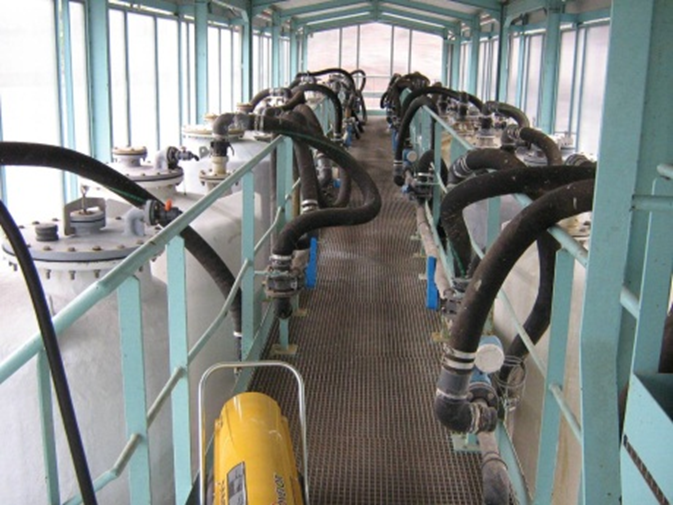
\includegraphics[width=0.9\linewidth]{III_A_3.png}
\caption{Les résines échangeuses d'ions de l'usine de traitement des eaux de Lodève (Hérault)}
\label{fig:usine_traitement_resines}
\end{figure}

Lors de la régénération des résines, il est possible de traiter la solution régénérante qui ressort du réservoir pour récupérer la substance polluante, soit pour une mise en déchet soit pour réutilisation. Ce processus est notamment très utilisé lors du traitement des eaux pour les mines d’uranium : l’uranium récupéré peut alors être utilisé ou vendu.
Ce type de traitement s’applique principalement à l’uranium dans le cadre des mines et il permet également de traiter des eaux contenant des métaux solubles, des sulfates, des nitrates, des cyanures, des halogénures… Le procédé est plus rarement utilisé pour les polluants organiques.
La majorité des coûts du traitement par résines échangeuses d’ions correspond à l’élution, aux coûts humains, matériels et de transport de la matière polluante.
Un demi équivalent temps plein est nécessaire pour surveiller les différents paramètres de suivi (débits d’eau, concentrations et paramètre de fonctionnements comme la consommation électrique…), pour remplacer les colonnes et nettoyer les filtres.
%(Tableau $III_A_1$)
% \begin{figure}[!ht]
% \centering
% 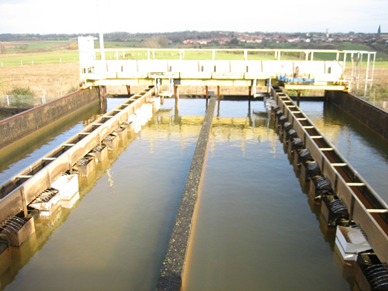
\includegraphics[]{III_A_1.png}
% \caption{Bassin de décantation}
% \label{fig:bassin_decantation}
% \end{figure}


\begin{center}
\begin{tabular}{ |c |c |}
\hline
 Tâche à réaliser & Temps nécessaire pour un fonctionnement hebdomadaire permanent \\ 
 \hline
 Nettoyage des filtres & 8 h / semaine \\ 
 \hline
 Changement des colonnes & 8,5 h / colonne / semaine  \\
 \hline
Analyses & 4h / semaine  \\
 \hline
\end{tabular}
\end{center}

Dans le cas d’une mine d’uranium, la régénération des résines saturées permet de récupérer et revendre l’uranium à un prix avoisinant 80 €/kg.
Le coût du matériel dépend directement du nombre de colonnes nécessaires et donc du débit d’eau à traiter : une colonne coûte 10 500 €.


Le coût du transport correspond notamment aux déplacements des résines vers les lieux de régénération et dépend donc de l’éloignement entre le site de traitement de l’eau et le site de régénération des résines.
L’ensemble des coûts de traitement pour un volume d’eau varie alors entre 0,10 et 0,50 €/$\text{m}^3$.

\paragraph{Traitement par zones humides}

A l’inverse des traitements précédents, les traitements passifs reposent sur des réactions chimiques à l’œuvre naturellement dans l’environnement. Ils ne nécessitent donc pas d’apport d’énergie supplémentaire. 

L’utilisation d’une zone humide (\textit{wetland} en anglais) constitue un moyen de traitement passif des effluents miniers. Le procédé est encore à l’étude et son emploi est encore très marginal en France : parmi les quinze stations de traitement des eaux françaises, une seule en est équipée. Un wetland désigne une étendue d’eau artificielle reproduisant les conditions d’une tourbière dans laquelle transitent des effluents miniers. 

L’abaissement des concentrations en polluants dans l’eau repose sur trois procédés conjoints. D’une part, des bactéries sulfato-réductrices sont nourries par la matière organique présentes dans la tourbe et permettent le maintien du caractère réducteur du milieu. Dans ces conditions, l’uranium tend à précipiter en uraninite insoluble. D’autre part, uranium et radium peuvent être sorbés sur la matière organique ou sur les fractions argileuses présentes dans la tourbe. Enfin, dans le cas des eaux d’exhaure riches en fer, la présence d’une couche d’eau à la surface de la tourbière favorise la précipitation d’oxy-hydroxydes de fer capables de fixer uranium et radium. 

Les coûts d’entretien d’une tourbière sont négligeables. Les seuls coûts significatifs lors de son fonctionnement sont ceux des analyses des eaux en sortie de la zone humide.


%(Image III_A_4)
\begin{figure}[H]
\centering
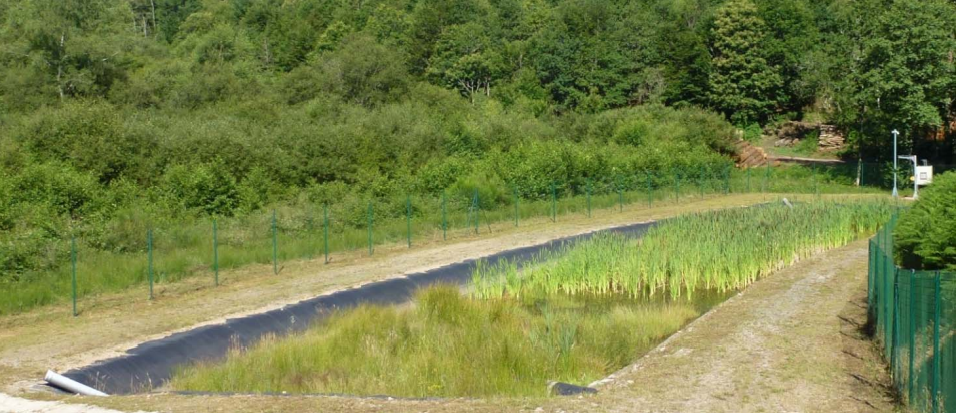
\includegraphics[width=0.8\linewidth]{III_A_4.png}
\caption{Une tourbière}
\label{fig:tourbiere}
\end{figure}


\paragraph{Pas de traitement : prélèvements et analyses}

Il est assez fréquent qu’aucun traitement ne soit nécessaire sur un site minier, lorsque le site est assez isolé ou bien lorsque le traitement qui était nécessaire lors de l’exploitation est devenu inutile (voir III.B). Le coût n’est cependant pas nul, il faut continuer les prélèvements et analyses pour vérifier en permanence que l’eau n’a effectivement pas à être traitée et pouvoir traiter rapidement si un phénomène imprévu présente des dangers (apparition d’un nouveau rejet, effet saisonnier...). Les prélèvements doivent être réalisés au moins une fois par semaine et impliquent donc un coût humain. Il faut également payer les laboratoires responsables des analyses de ces prélèvements.


Le coût est donc, même si aucun traitement n’est mis en place, non négligeable  par rapport au coût total de l’après mine. Avec ou sans traitement, les prélèvements et analyses réalisés dans l’ensemble de la filière après-mine représentent un investissement de 700 000 à 800 000 € par an.


Il est de même préférable de laisser les infrastructures en place après l'interruption d’un traitement, et de les entretenir régulièrement pour pouvoir recommencer le traitement si nécessaire, et permettre  une meilleure entente avec les associations et les locaux. 


\subsubsection{Comparaison, faisabilité}
Les trois méthodes de traitements discutées ci-dessus sont aujourd’hui utilisées en France. Bien qu’elles soient toutes les 3 non destructives, elles ne sont pas perçues de la même manière et présentent chacune certains avantages ou aspects contraignants importants à étudier pour savoir quel type de traitement utiliser sur chaque site.


\paragraph{Investissement et mise en place}

Les coûts détaillés à la partie précédente représentent principalement les OPEX (dépenses d’exploitation). Les CAPEX (dépenses d’investissement) représentent également une dépense conséquente qui s'additionnent à toute la gestion de l’après-mine. Ce type de dépense doit donc être pris en compte pour choisir un type de traitement plutôt qu’un autre.

Les CAPEX prennent en compte les dépenses liées aux infrastructures et à l’achat du gros matériel non remplacé pendant l’exploitation. Ce coût est équivalent pour ce qui concerne les traitements par précipitation et par zone humide, mais il est 4 à 5 fois plus important pour le traitement par résines échangeuses d’ions.

Il faut cependant également prendre en compte la durée de vie du matériel pour faire un retour sur investissement. Par exemple, si la construction d’un wetland demande un faible investissement, les travaux se réduisant souvent à quelques opérations de terrassement, la tourbe nécessaire à son fonctionnement semble devenir inefficace en quelques années. Or, l’approvisionnement en tourbe a un impact économique et environnemental important, puisque, l’exploitation industrielle de la tourbe française étant strictement réglementée, il peut être nécessaire de l’importer, notamment des pays baltes. 

L’impact environnemental des infrastructures est aussi à prendre en compte. Par exemple, alors que le traitement par précipitation nécessite la construction de nombreux bassins spacieux et pouvant empiéter sur l’environnement, le wetland s’insère dans le paysage, accueillant la végétation et permettant le développement d’une faune spécifique.

\paragraph{Exploitation et maintenance}

Les méthodes de traitement présentent chacune des avantages et inconvénients relatifs à leur exploitation. D’une part, leurs caractéristiques techniques ne leur permettent pas de prendre en charge les mêmes débits d’effluents. Le traitement par précipitation et coagulation-floculation-décantation est le plus productif, avec environ 200 $\text{m}^3$ traités par heure, mais aussi le plus flexible, avec une bonne capacité d’adaptation aux variations saisonnières du volume d’effluent entrant. 
Le traitement par résines échangeuses d’ions permet le traitement d’environ 100 $\text{m}^3$ d’effluent par heure et présente une bonne adaptabilité au débit grâce à la possibilité de placer les bouteilles en série ou en parallèle. Au contraire, le wetland ne traite que de très faibles débits, de l’ordre du $\text{m}^3$ par heure.

Le traitement par résines échangeuses d’ions est le traitement le plus efficace pour abattre la concentration en uranium de l’eau avec un rendement pouvant atteindre 95\% ou même 98\% lorsque les colonnes sont disposées en série.  Tout comme le procédé de précipitation, qui permet d’atteindre dans de bonnes conditions des rendements de 90\%, il est en mesure d’éliminer une large gamme de polluants grâce au recours à différentes résines. L’efficacité de ces deux traitements est en outre sensible aux caractéristiques chimiques de l’effluent, telles que son pH ou la présence de certains éléments. Pour le traitement par résines, la présence de précipités peut très fortement nuire au traitement. Un prétraitement, l’élution, est alors nécessaire et représente la majorité des coûts du traitement par résines. Le wetland est de nouveau la solution la moins efficace, l’abattage des concentrations en uranium et radium étant de l’ordre de 50 à 70\%.

Le traitement par résines met en jeu des réactions rapides qui permettent, sous réserve de bonnes conditions chimiques, un traitement rapide des eaux. A l’inverse, le traitement par précipitation repose sur une longue phase de décantation pouvant durer plusieurs jours. Les deux solutions de traitement actif présentent également des coûts importants en maintenance (transport des résines, manutention des colonnes, nettoyage préventif des cuves) et en réactifs tandis que l’utilisation du wetland ne requiert pas la présence permanente d’un opérateur. Les seuls coûts associés à son fonctionnement sont les coûts des analyses de l’eau en sortie.  Néanmoins, la durée d’efficacité du wetland semble courte : des données relevées en 2020 au bassin pilote de la mine d’Henriette ouvert en 2014 montrent que l’abattage des concentrations en polluants est moins important après cinq ans d’activité. 

En termes de coûts, les traitements par zones humides et par précipitation sont plus avantageux que celui par résine car l’investissement et l’élution sont trop coûteux, même en prenant en compte les éventuelles ventes après régénération de la résine.
%(Tableau III.A.2)


\begin{center}
\begin{tabular}{ |c |c |}
\hline
 Type de traitement & Coût d’exploitation en € / m3 \\ 
 \hline
 Précipitations & 0.20 à 0.50 \\ 
 \hline
 Résines échangeuses d’ions & 0.10 (avec revente du polluant) à 0.50  \\
 \hline
Zones humides & Négligeable  \\
 \hline
\end{tabular}
\end{center}

L’un des principaux enjeux de l’après-mine est de diminuer ces coûts car le traitement par résine est très avantageux lorsque le polluant peut être récupéré.

\paragraph{Gestion des déchets }

Les traitements produisent des déchets sous différentes formes qu’il est nécessaire de stocker où d’évacuer en respectant les normes et les sociétés locales.

Le traitement par zone humide engendre des tourbes saturées au bout de quelques années. La question de la gestion de cette matière organique chargée est encore à l’étude. En outre, l’utilisation d’un wetland peut entraîner le relargage des métaux fixés dans l’environnement avoisinant.
De même, le traitement par précipitation donne naissance à d’importants volumes de boues qui impliquent de nouveaux coûts de traitement ou de déshydratation. Il peut également augmenter les concentrations en sulfates dans l’eau. 

Au contraire, le traitement par résines échangeuses d’ions est très bien perçu par les associations car il permet de retirer définitivement un certain type de polluant du site minier. C’est notamment le cas pour les mines d’uranium : les associations qui se focalisent sur les dangers liés à l’uranium sont satisfaites par l’exportation de ce dernier vers d’autres lieux ou il va être traité puis revendu lors de la régénération des résines.

Cependant ce type de traitement provoque la création de nouveaux déchets, à l’extérieur du site minier, lorsque le polluant ne peut pas être réutilisé après avoir été récupéré lors de la régénération des résines. Le problème est donc dans ce cas le même que la gestion des déchets liés aux traitements par zones humides et précipitations.

Le traitement de l’eau par résine échangeuse d’ion est alors plus avantageux que les autres principalement dans le cas où le polluant peut être récupéré après régénération de la résine: le coût est diminué grâce à la revente et le processus ne produit presque pas de déchets.

Ne pas traiter une eau dont les teneurs en polluants sont en adéquation avec les normes en vigueur est aussi une solution pertinente sur les plans environnementaux et économiques, son coût se réduisant aux frais de contrôle et d’analyse des eaux. Cette solution pourrait également être pertinente dans le cas où l’évacuation de l’eau vers un cours d’eau met en jeu des dilutions importantes. Néanmoins, du fait de l’exacerbation de la dangerosité de l’uranium dans l’opinion collective, un traitement, même s’il est plus susceptible de dégrader la qualité de l’eau que de l’améliorer, est souvent préféré par les populations locales. De même, l’interruption d’un traitement des eaux est susceptible d’être mal accueillie par les riverains.

\subsubsection{Présentation des situations des autres pays}
\paragraph{Situation générale de mines d’uranium de chaque pays}
\paragraph{Les méthodes de traitement préférées par pays}

\subsection{Les traitements sont-ils toujours nécessaires ? Étude de cas du site de la Ribière}
\subsubsection{Présentation du site de La Ribière}
L’étude du traitement des eaux d’exhaure d’une mine nécessitait de se baser sur un exemple concret, et c’est pour cette raison que nous nous sommes penchés sur le site de la Ribière. 

Situé sur la commune de Domeyrot dans la Creuse, ce site a été exploité de 1959 à 1984 par la compagnie TCMF (\emph{Total Compagnie Minière France}), qui en a extrait 142,9 tonnes d’uranium sur l’ensemble de la durée d’exploitation. Pour récupérer cette quantité d’uranium, il a fallu extraire 628 kt d’une mine à ciel ouvert (MCO) d’une superficie de 17472 m². Il n’y a pas de travaux miniers souterrains à la Ribière.

Le traitement du minerai brut extrait a conduit, d’une part à l’uranium, et d’autre part à un volume important de résidus et de stériles miniers. Ainsi, une partie de ces résidus a été stockée sur le site, dans l’emplacement correspondant à l'ancienne mine à ciel ouvert, et pour une masse totale de 192 000 tonnes.

Ces résidus, placés en grande partie dans l’ancienne MCO, ont été traités de manière statique, par lixiviation \textit{in situ} entre 1982 et 1985. Il s'agissait d’un minerai pauvre en uranium, avec une concentration de l’ordre de 350 ppm. 

Puis, une fois cette phase de dépôt effectuée, le site est entré en phase de réaménagement entre 1991 et 1992, par son recouvrement avec une couche de stériles et de terre épaisse de 4 mètres et sa végétalisation (partielle). La surface est recouverte d’herbe étant donné que l’on ne peut pas laisser un système racinaire développé s’implanter, car cela favoriserait une infiltration trop importante d’eau.

Le site constitue un bassin versant d’altitude maximale 405 mètres, avec le ruisseau Le Verraux qui le longe dans sa partie inférieure, à un altitude de 348 mètres.

Désormais géré par Orano Mining, le site de la Ribière a été équipé d'appareils de mesure et de surveillance, notamment pour ce qui est de l’eau qui traverse le site. Ainsi sont répartis sur les 14 ha 4 points de surface pour la surveillance environnementale, et 9 piézomètres qui s’enfoncent dans le sol afin d’en avoir une vision détaillée, et notamment le profil géologique et hydrologique de la zone.

Selon Orano Mining, le site, qui ne dispose pas de station de traitement des eaux, respecte les normes environnementales en vigueur en termes de qualité des eaux à l’exutoire. La concentration en uranium mesurée est de $7,6 \cdot 10^{-6} $ mol/L et la dose mesurée est de $1,37$ Bq/L pour le $^{226}$Ra.

Nous nous proposons donc de mettre en œuvre deux modèles du site, hydrologique et géochimique, afin de confirmer ces mesures et d’obtenir une prévision de long terme quant au respect de ces normes. 

\subsubsection{Modèle géochimique et 1D}
\paragraph{Modélisation}


\paragraph{Résultats du modèle géochimique }

\subsubsection{Modèle hydrologique 2D}
\paragraph{Modélisation}

Pour proposer un modèle convaincant du site, il est nécessaire de s’intéresser aux flux hydrogéologiques. Nous avons pour cela utilisé un rapport hydrogéologique du site, daté de 2011. Nous nous sommes basés sur les relevés des 9 piézomètres du site et avons décidé de faire une modélisation en coupe. Cette coupe a été choisie puisqu’elle passe à la fois par la zone de résidus de traitement, par la rivière en contrebas, et par 5 piézomètres différents.

\begin{figure}[H]
    \centering
    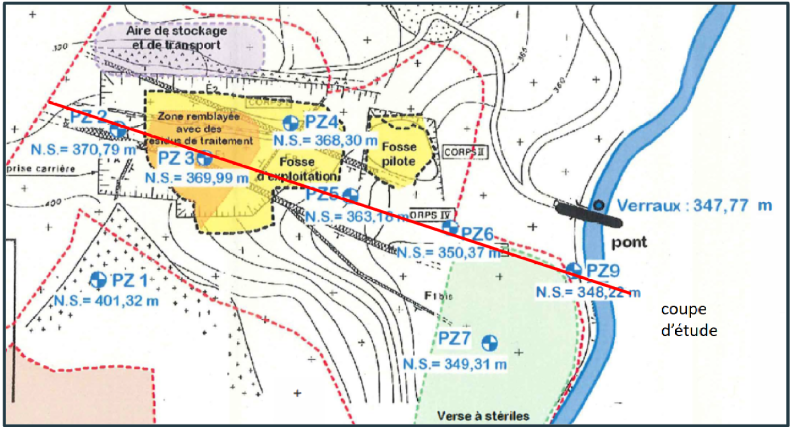
\includegraphics[width=0.8\linewidth]{III_B_3_1.png}
    \caption{Coupe réalisée pour l'étude du site (Orano)}
    \label{fig:coupe_ribiere}
\end{figure}



Les relevés piézométriques permettent de définir plusieurs zones. On note tout d’abord une zone de surface, composée d’une arène granitique, et de stériles miniers au dessus de la zone de résidus, d’une épaisseur moyenne de 4 m. Celle-ci est composée de deux faciès, un faciès sableux et un faciès boueux. Une zone de granite fracturé est également présente, en dessous de laquelle on trouve une zone de granite sain. Les résidus de traitement apparaissent donc comme localisés et situés proches d’une zone de granite fracturé. L’identification de ces différentes zones permet la création d’un maillage grâce au logiciel GMSH, et la modélisation du site grâce à HYTEC.

\begin{figure}[H]
    \centering
    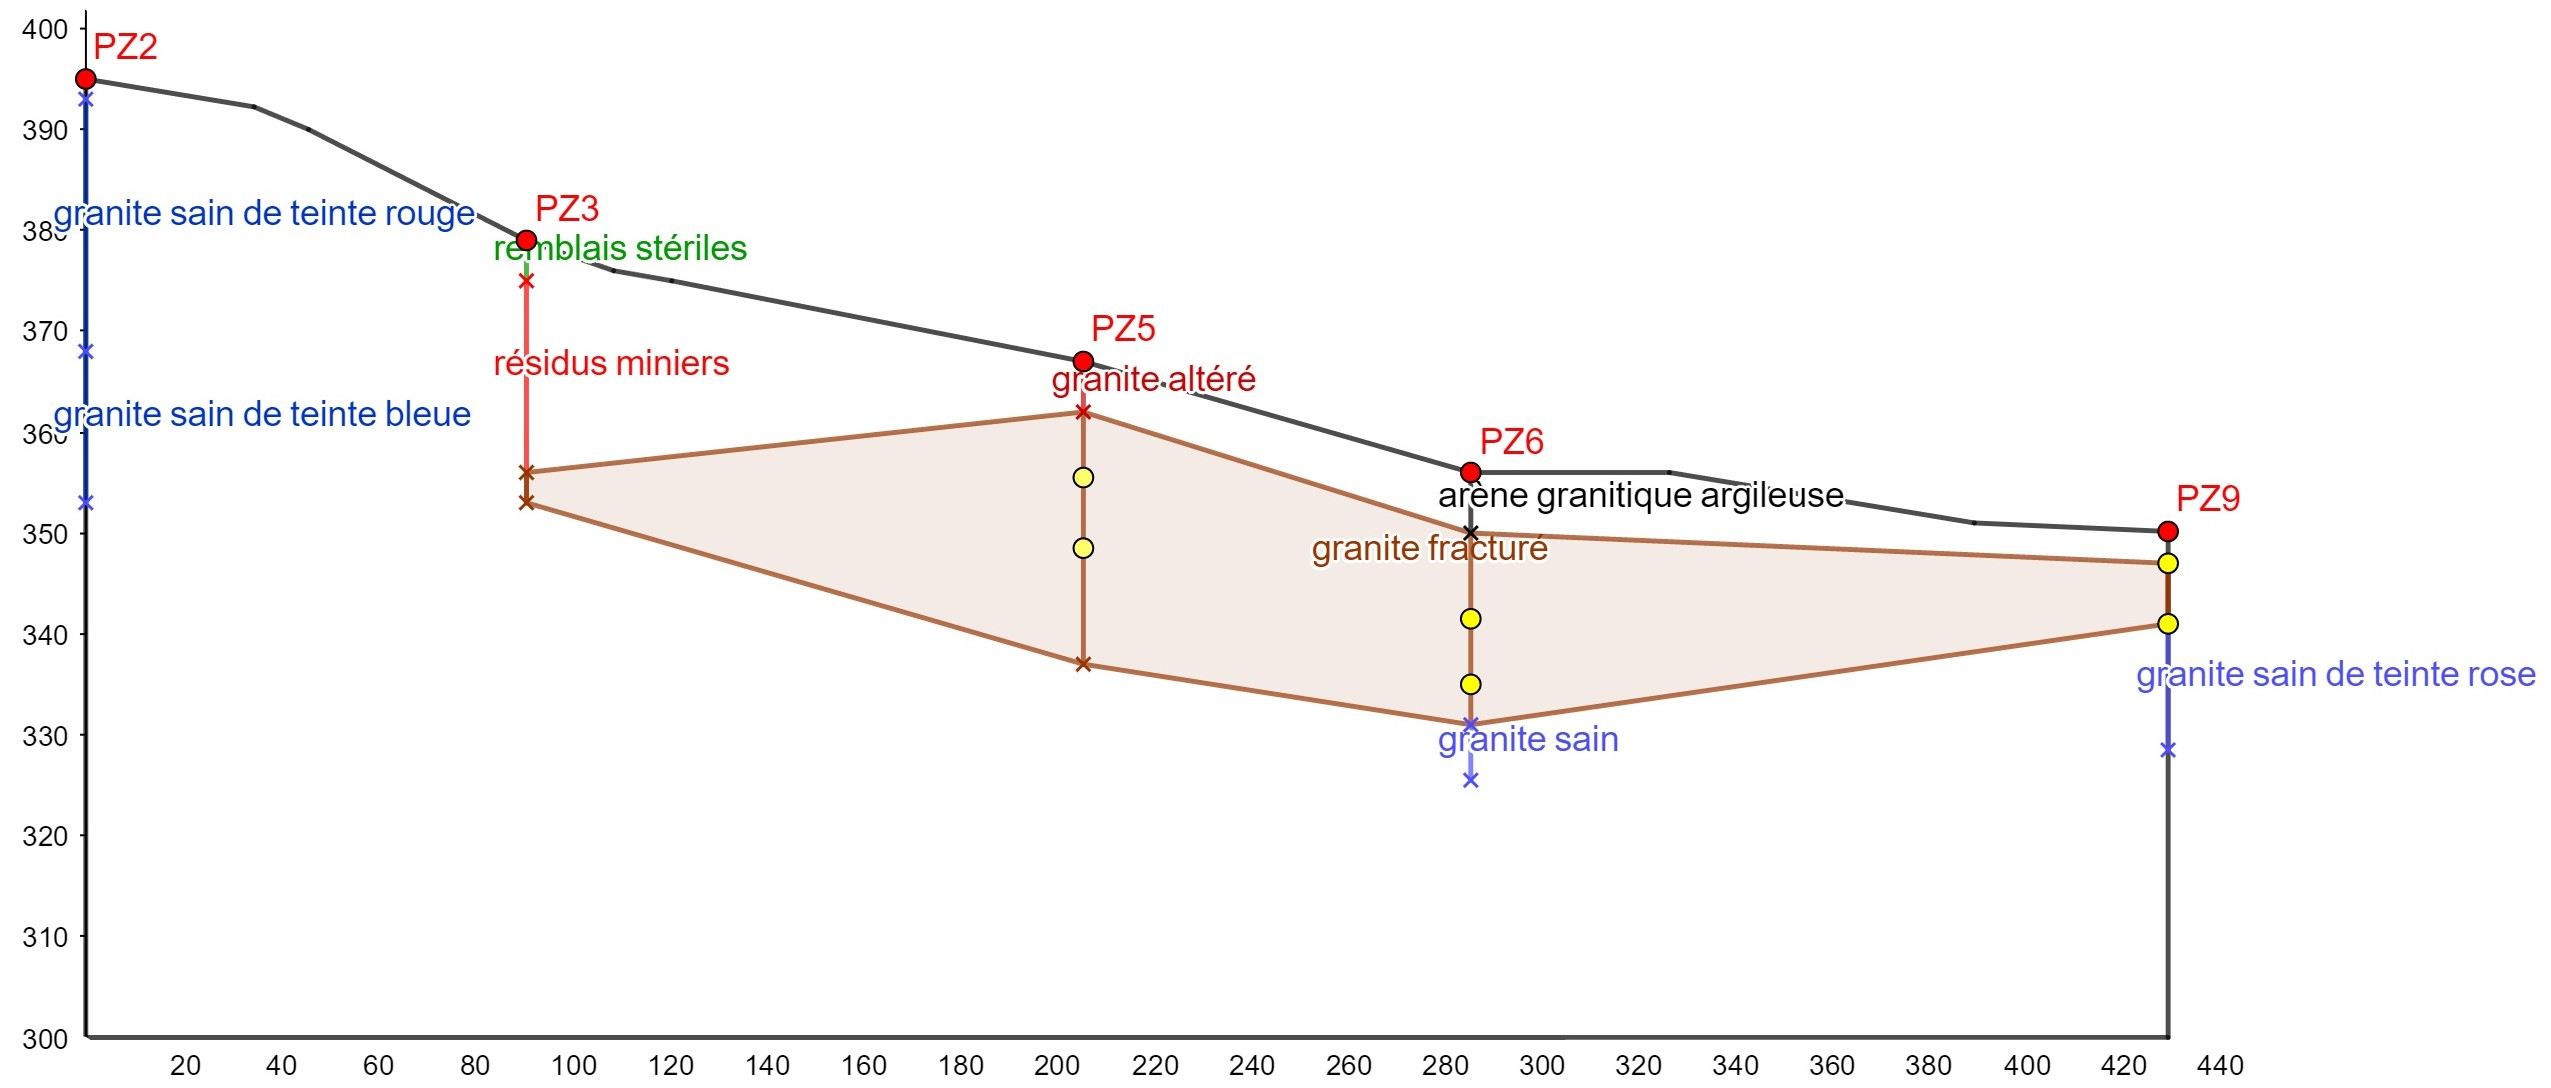
\includegraphics[width = 0.9\textwidth]{III_B_3_2.jpg} 
    \caption{Modélisation des différentes zones}
    \label{fig:zones_ribieres_geogebra}
\end{figure}


\begin{figure}[H]
    \centering
        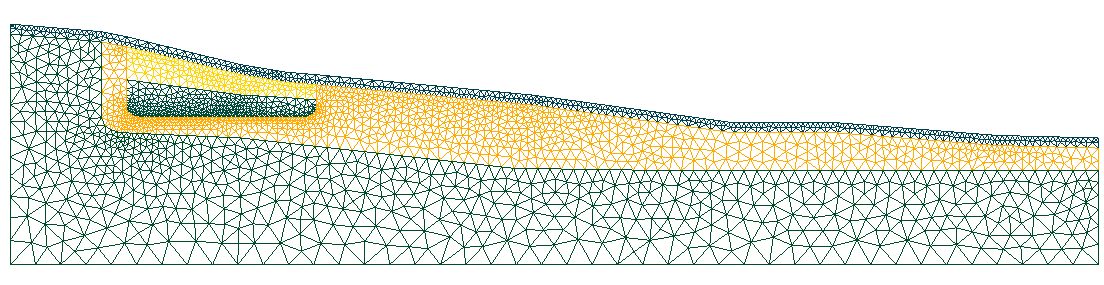
\includegraphics[width=0.9\textwidth]{III_B_3_3.png} 
        \caption{Maillage de la zone obtenu avec GMSH}
        \label{maillage_ribiere}
\end{figure}

Les relevés piézométriques permettent aussi de définir un niveau de charge: le piézomètre PZ2 indique une profondeur d’eau à environ 24 m, et le piézomètre PZ9 à 1 m, ce qui correspond au Verraux.

Les données météorologiques montrent des précipitations effectives (c’est à dire la différence entre les précipitations totales et l’évapotranspiration) variables au cours de l’année : en effet, on remarque que les mois de novembre,décembre, janvier et mars correspondent à de hautes valeurs de précipitations effectives, alors qu’elles sont presque nulles le reste de l’année. Ceci permet donc de modéliser les saisons et les variations de précipitations, et met en évidence l’importance de la couche de surface, qui sert d’interface pour les transferts.


\begin{figure}[H]
    \centering
    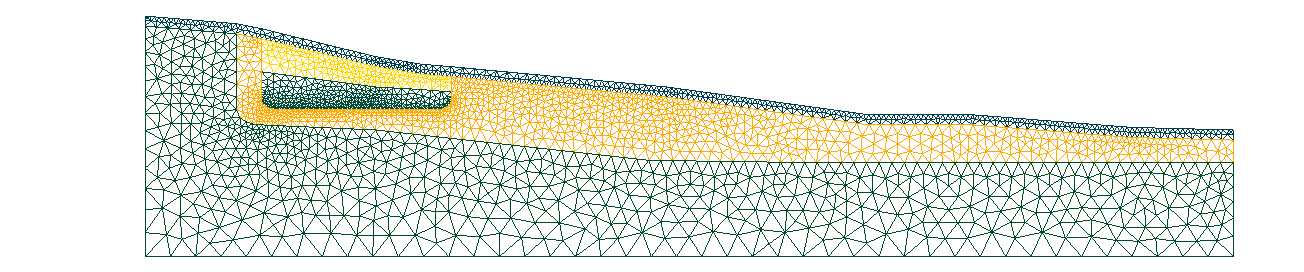
\includegraphics[width=0.8\linewidth]{III_B_3_4.png}
    \caption{Précipitations annuelles sur le site de la Ribière (Orano)}
    \label{fig:precipitations_ribiere}
\end{figure}

\paragraph{Résultats}

Les modélisations montrent l’importance de la perméabilité et de la porosité des différentes zones, puisque de faibles variations induisent des comportements différents à long terme. Il est donc nécessaire d’avoir des valeurs les plus précises possibles et les plus représentatives du site. En effet, un gradient de perméabilité trop élevé, ou bien des discontinuités de perméabilité peuvent engendrer des comportements non représentatifs, comme une remontée du traceur dans les résidus en surface.

La détermination du temps de résidence peut se faire de différentes façons. Une approximation linéaire permet un calcul d’ordre de grandeur : une modélisation par deux zones, une zone de résidus et une de granite fracturé, donne un temps de résidence d’environ 15 ans. La solution analytique donne également le même ordre de grandeur. Enfin, le modèle hydrogéologique montre l’évolution du traceur des résidus : on obtient ici un temps de résidence de 25 ans.

\begin{figure}[!h]
    \centering
    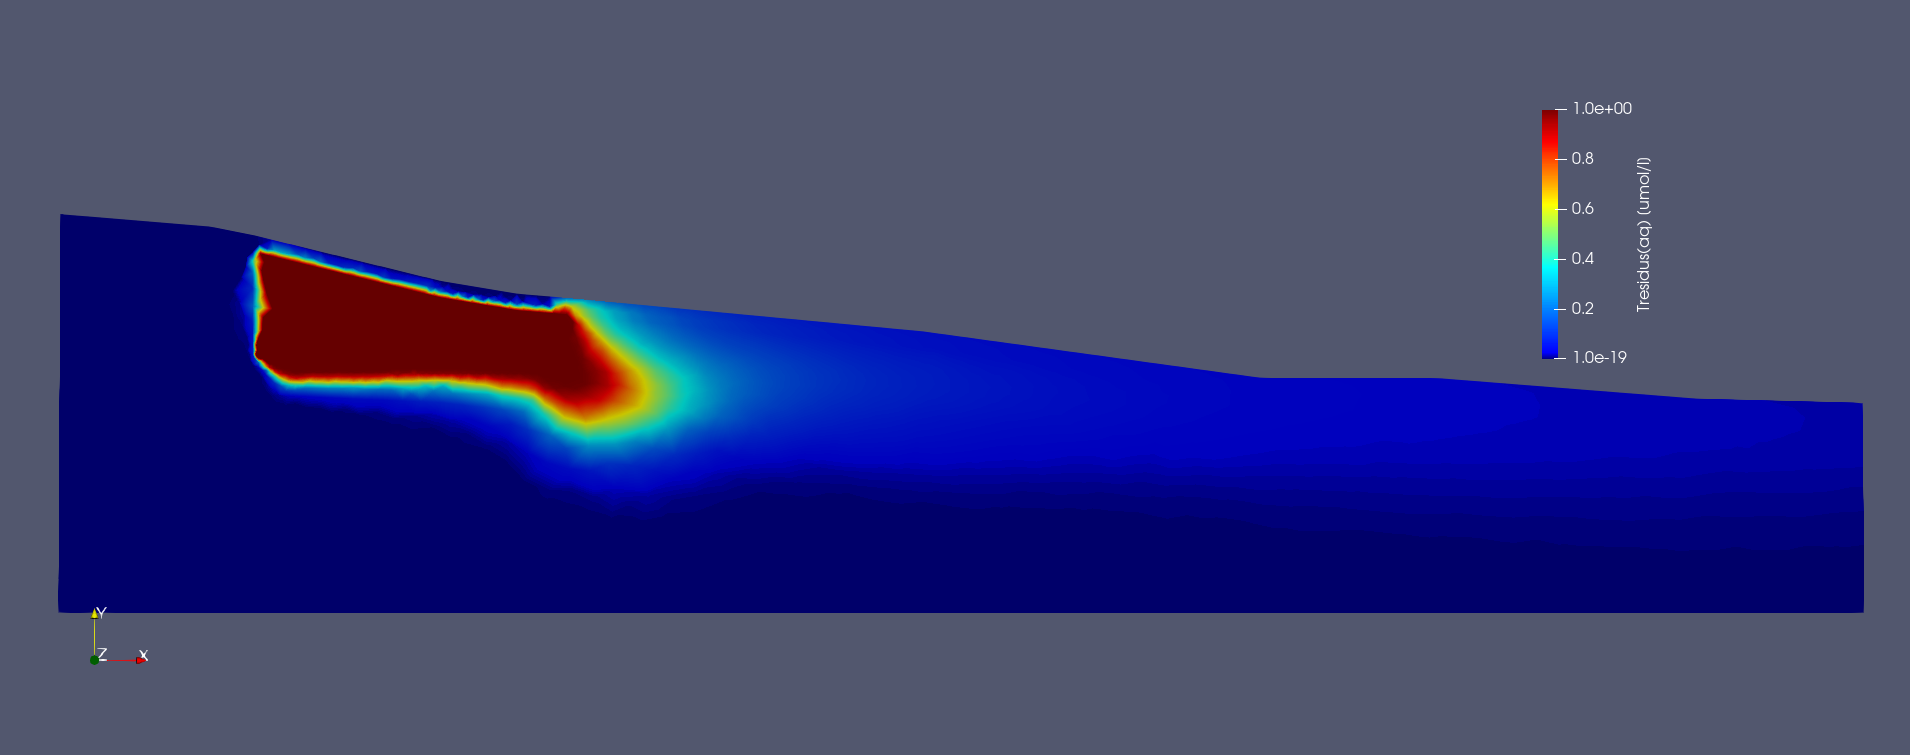
\includegraphics[width=0.8\linewidth]{III_B_3_5.png}
    \caption{Résultat de la simulation du modèle hydrogéologique après 25 ans}
    \label{hytec_hydro_25ans}
\end{figure}

Ces résultats sont à nuancer, puisqu’à ce stade aucun modèle chimique n’a été intégré. De plus, certaines données non renseignées permettraient d’aller plus loin. Il serait possible d’affiner les bords de la fosse à résidus: nous l’avons modélisé par un trapèze, mais il est très probable que les pentes de la fosse aient une forme de gradins, afin d’assurer la stabilité de la zone. La donnée de la hauteur et de la largeur des marches permettrait une modélisation plus fine.

La nature des résidus est également peu connue. Il y a une alternance entre les deux faciès, mais la proportion réelle de chaque n’est pas renseignée. Or ces deux zones ont des comportements hydrogéologiques très différents, avec des porosité et perméabilités différentes. Une analyse géochimique des résidus pourrait donc être réalisée. De plus, seul un unique piézomètre est présent dans cette zone, ce qui induit des incertitudes : on ne dispose que des données en un point pour une zone de 80 m de long et d’environ 20m de profondeur.

Le granite fracturé aux alentours n’est pas non plus très bien connu. Des analyses seraient nécessaires pour déterminer ses caractéristiques, afin de les comparer avec celles du granite sain. Le fait que la zone soit fracturée va en effet modifier drastiquement le comportement hydrologique, puisqu’il s’agit de la zone la plus en contact avec les résidus miniers.

\paragraph{Modèle hydrogéochimique}

Une fois le modèle hydrogéologique et le modèle chimique établi, nous avons pu concevoir un nouveau modèle, prenant en compte la dynamique des flux hydrologiques et les interactions chimiques entre les éléments mis en jeu. Ceci introduit de nouvelles sensibilités, puisque l’augmentation ou la diminution de la concentration ou de la distribution d’un élément peut impacter tout le modèle. On obtient donc un modèle à la fois très sensible aux caractéristiques des roches, mais aussi à des données chimiques comme le pH.

Il a fallu néanmoins interpréter certaines données. Des relevés et analyses chimiques dans les différentes zones mises en jeu pourraient être réalisées pour évaluer précisément les compositions et concentrations en les différentes espèces. Par exemple, les taux précis en gypse ne sont pas connus partout.


\subsubsection{Conclusion pour le site}

\subsection{Le radon, un gaz volatile}

\newpage
\section{Synthèse des enjeux}
\subsection{Aspect socio-économique du traitement de l’eau}
\subsection{Ouverture à l’internationale}

\section*{Conclusion}

%%%%%% ANNEXES %%%%%%%
\newpage
\appendix
\pagenumbering{roman}
\titleformat{\section}
    {\Large\bfseries}
    {Annexe \thesection \: -}
    {0.5 em}
    {}
\newpage
\section{Références bibliographiques}
\printbibliography[header = none]

\newpage
\section{Figures utiles}


\newpage
\section{Code HYTEC Utilisé }

% c'est beau hein
\lstinputlisting[language=hytec, caption = Modèle hydrogéologique outdated]{modele-13.htc}
\newpage
\section{Résultats des simulations numériques HYTEC}


\newpage
\listoffigures

\end{document}
